% XRB-pilot: technical report (English) -- main file.
% Compile with:  latexmk -pdf main.tex   (run inside report_en/)
% Every number in this report is read from files committed in the repository (results/, data/, reports/);
% comments starting with "% CHECK:" mark places where the repository text and the CSV/code disagree.
\documentclass[11pt,a4paper]{report}

% ------------------------------------------------------------------ page, fonts
\usepackage[a4paper,margin=1in,headheight=14pt]{geometry}
\usepackage[T1]{fontenc}
\usepackage{lmodern}
\usepackage[utf8]{inputenc}
\usepackage{CJKutf8}  % Traditional Chinese terms in the glossary (bsmi font)
\usepackage{microtype}
\usepackage{xcolor}
\usepackage{graphicx}
\usepackage{booktabs}
\usepackage{longtable}
\usepackage{array}
\usepackage{multirow}
\usepackage{makecell}
\usepackage{tabularx}
\usepackage{siunitx}
\usepackage{amsmath}
\usepackage{amssymb}
\usepackage{mathtools}
\usepackage{bm}
\usepackage{enumitem}
\usepackage{float}
\usepackage{placeins}
\usepackage{pdflscape}  % landscape pages (rotated in the PDF viewer) for very wide repository figures
\usepackage{afterpage}
\usepackage{caption}
\usepackage{subcaption}
\usepackage[authoryear,round,sort]{natbib}
\usepackage[most]{tcolorbox}
\usepackage{algorithm}
\usepackage{algpseudocode}
\usepackage{tikz}
\usetikzlibrary{positioning,arrows.meta,fit,calc,shapes.geometric,shapes.misc,backgrounds,decorations.pathreplacing,matrix}
% ------------------------------------------------------------------ flowchart styles (figures/flowcharts/*.tex)
% node kinds: data/sample (amber), processing/features (green), model/evaluation (blue), reused from an earlier version
% (dashed grey), implementation check (chamfered); comparison status: primary/secondary/descriptive; verdicts.
\tikzset{
  fc/.style={rounded corners=2pt, align=center, font=\scriptsize, inner sep=2.2pt,
             execute at begin node={\hyphenpenalty=10000\exhyphenpenalty=10000\relpenalty=10000\binoppenalty=10000\relax}},
  fc data/.style={fc, rounded corners=0pt, draw=tagexp, fill=tagexp!9},
  fc proc/.style={fc, draw=tagsec, fill=tagsec!9},
  fc model/.style={fc, draw=tagprim, fill=tagprim!8},
  fc old/.style={fc, draw=inkgrey!55, dashed, fill=white, text=inkgrey},
  fc gate/.style={fc, chamfered rectangle, chamfered rectangle xsep=1.4mm, draw=inkgrey, fill=boxgrey},
  fc dec/.style={fc, diamond, aspect=2.4, draw=inkgrey, fill=white, inner sep=0.6pt},
  fc prim/.style={fc, draw=tagprim, line width=0.9pt, fill=white},
  fc sec/.style={fc, draw=tagsec, line width=0.6pt, fill=white},
  fc descr/.style={fc, draw=tagdesc, dashed, fill=white},
  fc yes/.style={fc, draw=green!40!black, line width=0.6pt, fill=green!14},
  fc part/.style={fc, draw=green!40!black, line width=0.6pt, fill=white,
                  path picture={\fill[green!40!black!55] (path picture bounding box.south west) rectangle ([xshift=1.3mm]path picture bounding box.north west);}},
  fc no/.style={fc, draw=inkgrey, fill=black!7},
  fc none/.style={fc, draw=tagdesc, dashed, fill=white},
  fc arr/.style={-{Stealth[length=1.7mm]}, semithick, inkgrey},
  fc head/.style={font=\scriptsize\bfseries, text=inkgrey, align=center},
  fc ver/.style={draw=inkgrey, fill=inkgrey, text=white, font=\tiny\bfseries\sffamily, rounded corners=1pt, inner sep=1.1pt,
                 anchor=south west, minimum height=0pt, text width=, align=left},
  fc tag/.style={font=\tiny\sffamily},
  fc note/.style={font=\tiny, text=inkgrey, align=flush left, inner sep=1pt,
               execute at begin node={\hyphenpenalty=10000\exhyphenpenalty=10000\relax}},
}
% status tags inside flowchart comparison nodes
\newcommand{\fcP}{\textcolor{tagprim}{\textsf{\tiny\bfseries PRIMARY}}}
\newcommand{\fcS}{\textcolor{tagsec}{\textsf{\tiny\bfseries SECONDARY}}}
\newcommand{\fcD}{\textcolor{tagdesc}{\textsf{\tiny\bfseries DESCRIPTIVE}}}
\newcommand{\fcX}{\textcolor{tagexp}{\textsf{\tiny\bfseries EXPLORATORY}}}
\newcommand{\fcH}{\textcolor{tagpost}{\textsf{\tiny\bfseries POST HOC}}}
% one-line legends for the flowcharts; argument = west end of the legend
\newcommand{\fclegendnodes}[1]{%
  \begin{scope}[every node/.append style={font=\tiny}]
  \node[fc data, minimum width=3.2mm, minimum height=2.2mm, inner sep=0pt, anchor=west] (lg1) at (#1) {};
  \node[right=1pt of lg1] (lt1) {new data};
  \node[fc proc, minimum width=3.2mm, minimum height=2.2mm, inner sep=0pt, right=2.5mm of lt1] (lg2) {};
  \node[right=1pt of lg2] (lt2) {new processing or features};
  \node[fc model, minimum width=3.2mm, minimum height=2.2mm, inner sep=0pt, right=2.5mm of lt2] (lg3) {};
  \node[right=1pt of lg3] (lt3) {new model or evaluation};
  \node[fc old, minimum width=3.2mm, minimum height=2.2mm, inner sep=0pt, right=2.5mm of lt3] (lg4) {};
  \node[right=1pt of lg4] (lt4) {reused};
  \node[fc gate, minimum width=4mm, minimum height=2.2mm, inner sep=0pt, right=2.5mm of lt4] (lg5) {};
  \node[right=1pt of lg5] (lt5) {implementation check};
  \end{scope}}
\newcommand{\fclegendverdicts}[1]{%
  \begin{scope}[every node/.append style={font=\tiny}]
  \node[fc prim, minimum width=3.2mm, minimum height=2.2mm, inner sep=0pt, anchor=west] (lv1) at (#1) {};
  \node[right=1pt of lv1] (lu1) {primary};
  \node[fc sec, minimum width=3.2mm, minimum height=2.2mm, inner sep=0pt, right=1.8mm of lu1] (lv2) {};
  \node[right=1pt of lv2] (lu2) {secondary};
  \node[fc descr, minimum width=3.2mm, minimum height=2.2mm, inner sep=0pt, right=1.8mm of lu2] (lv3) {};
  \node[right=1pt of lv3] (lu3) {descriptive/exploratory};
  \node[fc yes, minimum width=3.2mm, minimum height=2.2mm, inner sep=0pt, right=3.5mm of lu3] (lv4) {};
  \node[right=1pt of lv4] (lu4) {detected};
  \node[fc part, minimum width=3.2mm, minimum height=2.2mm, inner sep=0pt, right=1.8mm of lu4] (lv5) {};
  \node[right=1pt of lv5] (lu5) {partly detected};
  \node[fc no, minimum width=3.2mm, minimum height=2.2mm, inner sep=0pt, right=1.8mm of lu5] (lv6) {};
  \node[right=1pt of lv6] (lu6) {not detected};
  \node[fc none, minimum width=3.2mm, minimum height=2.2mm, inner sep=0pt, right=1.8mm of lu6] (lv7) {};
  \node[right=1pt of lv7] (lu7) {no decision};
  \end{scope}}

\usepackage{fancyhdr}
\usepackage[hidelinks=false,colorlinks=true,linkcolor=blue!50!black,citecolor=green!35!black,urlcolor=blue!60!black,
            bookmarksnumbered=true,hypertexnames=false,pdftitle={XRB-pilot technical report},pdfauthor={TODO}]{hyperref}
\usepackage{xurl}
\usepackage[capitalise,noabbrev]{cleveref}

\graphicspath{{./}}
\setlength{\parindent}{0pt}
\setlength{\emergencystretch}{2.5em}
\setlength{\parskip}{0.55em}
\setlist{itemsep=0.15em,topsep=0.3em}
\captionsetup{font=small,labelfont=bf,format=plain,justification=justified}
\captionsetup[sub]{font=footnotesize}
\sisetup{group-separator={,},group-minimum-digits=4}
\DeclareSIUnit\count{count}
\DeclareSIUnit\PCU{PCU}
\renewcommand{\arraystretch}{1.12}
\setcounter{tocdepth}{2}
\setcounter{secnumdepth}{3}

\pagestyle{fancy}
\fancyhf{}
\fancyhead[L]{\small\nouppercase{\leftmark}}   % full header width for the chapter title (long titles collided with a right header)
\fancyfoot[L]{\footnotesize\color{gray}XRB-pilot technical report}
\fancyfoot[C]{\thepage}
\renewcommand{\headrulewidth}{0.3pt}

% ------------------------------------------------------------------ cleveref names
\crefname{algorithm}{Algorithm}{Algorithms}
\crefname{equation}{Eq.}{Eqs.}
\Crefname{equation}{Equation}{Equations}
\crefname{appendix}{Appendix}{Appendices}

% ------------------------------------------------------------------ colours and tags
\definecolor{bhblue}{HTML}{2A78D6}
\definecolor{nsorange}{HTML}{EB6834}
\definecolor{aqua}{HTML}{1BAF7A}
\definecolor{inkgrey}{HTML}{52514E}
\definecolor{boxgrey}{HTML}{F4F3EF}
\definecolor{tagprim}{HTML}{1F4E9A}
\definecolor{tagsec}{HTML}{3C6E3C}
\definecolor{tagexp}{HTML}{8A5A00}
\definecolor{tagpost}{HTML}{9B2D2D}
\definecolor{tagdesc}{HTML}{52514E}

\newcommand{\tagbox}[2]{\tcbox[on line,boxsep=0pt,left=2pt,right=2pt,top=1pt,bottom=1pt,colback=#1!8,colframe=#1,boxrule=0.4pt,arc=1pt]{\textsf{\scriptsize\color{#1}#2}}}
\newcommand{\Primary}{\tagbox{tagprim}{PRIMARY}}
\newcommand{\Secondary}{\tagbox{tagsec}{SECONDARY}}
\newcommand{\Exploratory}{\tagbox{tagexp}{EXPLORATORY}}
\newcommand{\PostHoc}{\tagbox{tagpost}{POST HOC}}
\newcommand{\Descriptive}{\tagbox{tagdesc}{DESCRIPTIVE}}
\newcommand{\Detected}{\textbf{detected} (95\% CI excludes 0)}
\newcommand{\DetectedP}{\textbf{detected} ($p<0.05$)}
\newcommand{\NotDetected}{\textbf{not detected} under the pre-registered criterion}

% numbers with intervals: \ci{+0.264}{+0.048}{+0.455}
\newcommand{\ci}[3]{$#1$~$[#2,\,#3]$}
% file names and code identifiers: typewriter, robust in captions, line breaks allowed after "_" and "/"
\ExplSyntaxOn
\tl_new:N \l_xrb_path_tl
\DeclareRobustCommand{\file}[1]{\group_begin: \ttfamily
  \tl_set:Nn \l_xrb_path_tl {#1}
  \tl_replace_all:Nnn \l_xrb_path_tl {/} {/\allowbreak}
  \tl_replace_all:Nnn \l_xrb_path_tl {.} {.\allowbreak}
  \cs_set:Npn \_ {\textunderscore\allowbreak}
  \tl_use:N \l_xrb_path_tl \group_end:}
\DeclareRobustCommand{\code}[1]{\group_begin: \ttfamily
  \tl_set:Nn \l_xrb_path_tl {#1}
  \tl_replace_all:Nnn \l_xrb_path_tl {.} {.\allowbreak}
  \tl_replace_all:Nnn \l_xrb_path_tl {,} {,\allowbreak}
  \cs_set:Npn \_ {\textunderscore\allowbreak}
  \tl_use:N \l_xrb_path_tl \group_end:}
\ExplSyntaxOff
\newcommand{\zh}[1]{\begin{CJK}{UTF8}{bsmi}#1\end{CJK}}
\newcommand{\BH}{BH}
\newcommand{\NS}{NS}

% ------------------------------------------------------------------ maths
\newcommand{\vect}[1]{\bm{#1}}
\newcommand{\Xm}{\bm{X}}
\newcommand{\yv}{\bm{y}}
\newcommand{\gv}{\bm{g}}
\newcommand{\wv}{\bm{w}}
\newcommand{\shat}{\hat{\bm{s}}}
\newcommand{\xv}{\bm{x}}
\newcommand{\bv}{\bm{\beta}}
\newcommand{\indic}[1]{\mathbf{1}\!\left[#1\right]}
\newcommand{\R}{\mathbb{R}}
\DeclareMathOperator*{\argmax}{arg\,max}
\DeclareMathOperator*{\argmin}{arg\,min}
\DeclareMathOperator{\BA}{BA}
\DeclareMathOperator{\AUC}{AUC}
\DeclareMathOperator{\sinc}{sinc}
\DeclareMathOperator{\sgn}{sgn}
\DeclareMathOperator{\Real}{Re}
\DeclareMathOperator{\median}{median}
\DeclareMathOperator{\logit}{logit}
\DeclareMathOperator{\Var}{Var}

% ------------------------------------------------------------------ boxes
\newtcolorbox{glance}[1]{enhanced,breakable,colback=boxgrey,colframe=inkgrey,boxrule=0.5pt,arc=1.5pt,
  title={Phase at a glance: #1},fonttitle=\bfseries\sffamily,coltitle=white,colbacktitle=inkgrey,left=6pt,right=6pt}
\newtcolorbox{keybox}[1]{enhanced,breakable,colback=white,colframe=tagprim,boxrule=0.5pt,arc=1.5pt,
  title={#1},fonttitle=\bfseries\sffamily\small,coltitle=tagprim,colbacktitle=tagprim!8,left=6pt,right=6pt}
\newtcolorbox{cautionbox}[1]{enhanced,breakable,colback=tagpost!3,colframe=tagpost,boxrule=0.5pt,arc=1.5pt,
  title={#1},fonttitle=\bfseries\sffamily\small,coltitle=tagpost,colbacktitle=tagpost!8,left=6pt,right=6pt}

\algrenewcommand\algorithmicrequire{\textbf{Input:}}
\algrenewcommand\algorithmicensure{\textbf{Output:}}

% ------------------------------------------------------------------ title
\title{\textbf{Can a single X-ray observation tell a black hole from a neutron star\\in a source never seen in training?}\\[0.6em]
\large Leakage-safe, pre-registered tests with RXTE, MAXI and NICER\\(the XRB-pilot project, versions v1--v14)\\[0.4em]
\normalsize Technical report}
\author{TODO: author name \\ Advisor: TODO: advisor name}
\date{Report compiled on \today\\[0.3em]\small Repository \url{https://github.com/Chipwwwwww/XRB-pilot}, branch \texttt{master}, analysis commit \texttt{d9730c9}}

\begin{document}
\pagenumbering{roman}
\begin{titlepage}
\maketitle
\thispagestyle{empty}
\end{titlepage}

% =====================================================================================================
\chapter*{Abstract}\addcontentsline{toc}{chapter}{Abstract}
% =====================================================================================================
Can a single X-ray observation tell whether an accreting compact object is a black hole (BH) or a neutron star (NS), for a source
that the classifier has never seen? The XRB-pilot project (versions v1--v14) answered this question with a strict design:
dynamically confirmed BHs and burst- or pulse-confirmed NSs only; leave-one-source-out evaluation; source-level metrics with a
class-stratified source bootstrap; one or a few pre-registered primary comparisons per version, judged by whether the 95\%
interval excludes zero; and frozen models, rules and pipelines for every test on new data.

Using RXTE/PCA spectra of 31 sources (7 BH, 24 NS), a single 5--25\,keV spectrum classifies unseen sources well above chance
(source balanced accuracy 0.80--0.87, source AUC 0.88--0.95), but essentially all of the information is in two count-space
hardness ratios: the full spectral shape, intensity, 3--5 and 25--60\,keV bands, flexible algorithms with nested selection, 17 times
more observations per source and 15 additional sources add nothing detectable to the ranking of unseen sources. Variability-defined states show why: the colour
classifier separates BHs from NSs in soft states (observation-level AUC 0.954) but not in hard states (0.646; difference
$+0.31$ [$+0.10$, $+0.51$]). Inside the hard state, 0.016--4\,Hz variability measured with cross-detector cospectra adds
information: $+0.26$ [$+0.05$, $+0.46$] in AUC on the RXTE sample, consistently positive on NICER, $+0.15$ [$+0.03$, $+0.26$] when
RXTE and NICER are pooled (86 sources, 16 dynamically confirmed BHs; not an independent confirmation), and $+0.18$
[$+0.05$, $+0.34$] in a prospective test with a frozen pipeline and a pre-chosen random forest on new NICER observations. At fixed
colour the characteristic frequency of BH variability is lower by 0.3--0.6\,dex in every data set but one, with pooled $p=0.0012$
but non-significant single prospective tests. A burst catalogue, persistent BHs, event-mode frequencies up to 1\,kHz and MAXI/GSC
light curves (including an exact reproduction of a published classifier) qualify these results. All prospective confirmations are
at the observation level on the same 16 BHs; a source-level test on new BH transients is the necessary next step. This report
documents every phase, the full mathematics of features, models and statistics, and the mapping from the archived data to the
machine-learning matrices; it re-runs no analysis and every number is read from files committed in the repository.

% stub 00_executive_summary

\tableofcontents
\listoffigures
\listoftables
% stub 00_notation

\clearpage
\pagenumbering{arabic}

% stub 01_introduction

% =====================================================================================================
\chapter{Data sources and physical feature extraction}\label{ch:features}
% =====================================================================================================

This chapter defines, once, every input quantity used anywhere in the project: where the raw data come from, how a raw
file becomes a number, in which unit, by which function of the code, and what happens to non-positive or missing values.
The phase chapters (\cref{ch:phase1,ch:phase2,ch:phase3,ch:phase4,ch:phase5,ch:phase6}) refer back here and only state
differences. When the description in a repository report and the code differ, the code is followed and the difference
is flagged with a \texttt{\% CHECK} comment in the \LaTeX{} source.

% -----------------------------------------------------------------------------------------------------
\section{Instruments, data modes and catalogues}\label{sec:instruments}
% -----------------------------------------------------------------------------------------------------

\Cref{tab:instruments} lists every data product that enters a model or a test. All raw files were obtained by scripts;
every download is recorded with its URL, size in bytes and SHA256 in \file{logs/downloads.jsonl} (50\,773 records,
\cref{app:reproduction}). Raw data are not in git (\file{data/raw/} is ignored, large sets live outside the repository
under \file{~/xrb-pilot-data/}).

\begin{table}[htbp]
\centering\small
\caption[Instruments, data modes and catalogues]{Instruments, data modes and catalogues used in the project. ``Versions''
gives where the product enters a model or test. Band and resolution are those actually used by the code (not the
instrument limits). Code: the function that reads or processes the product.}
\label{tab:instruments}
\begin{tabularx}{\textwidth}{@{}p{3.3cm}p{1.5cm}X p{3.1cm}@{}}
\toprule
Product & Versions & What is used & Code \\
\midrule
RXTE/PCA Standard-2 Standard Products (\texttt{xp*\_s2.pha}, \texttt{\_b2.pha}, \texttt{.rsp}) & v1--v8, v10 &
129-channel total and \texttt{pcabackest} background spectra summed over the PCUs listed in the \texttt{ROWID} keywords;
5--25\,keV (3--25\,keV in v3b); response for the same PCU combination & \file{spectra.py}: \code{read\_pha},
\code{read\_rsp}, \code{net\_spectrum}; \file{04\_fetch\_process.py} \\
RXTE/PCA Standard-1 (\texttt{pca/FS46\_*}) & v2--v10 & 0.125\,s light curves per PCU (\texttt{XeCntPcu0--4}), plus array
rates \texttt{VpCnt}, \texttt{RemainingCnt}, \texttt{VLECnt}; 128\,s rows of 1024 bins & \code{spectra.std1\_rates};
\file{v5lib.py}; \file{v6lib.py}; \file{v7lib.py} \\
RXTE/PCA event mode (\texttt{pca/SE*.evt.gz}) & v8c & Events with \texttt{TIME}, \texttt{PCUID}; modes
\texttt{E\_\{n\}us\_\{m\}M\_0\_\{k\}s}; binned at $2^{-12}$\,s & \file{v8lib.py}: \code{read\_events},
\code{hf\_features} \\
RXTE/HEXTE cluster~B Standard Products (\texttt{xh*\_s1.pha}, \texttt{\_b1.pha}) & v4b3 & Net 25--40 and 40--60\,keV
count rates & \file{19\_v4b3\_hexte.py} \\
RXTE \texttt{MissionLongData} catalogues; HEASARC TAP \texttt{xtemaster} & v1--v8 & Observation lists: \texttt{OBSID},
\texttt{TIME}, \texttt{EXPOSURE}, \texttt{STD1RATE}, \texttt{RA}, \texttt{DEC}, \texttt{NPCU} & \file{03\_select\_observations.py},
\file{20\_v4b2\_select.py}, \file{41\_v8b\_select.py} \\
MAXI/GSC standard products, 1-day light curves & v7c, v8d, v9c & Photon fluxes in 2--4, 4--10, 10--20\,keV &
\file{38\_v7c2\_select.py} \\
de Beurs et al.\ (2022) processed data (GitHub, commit \texttt{488b785}) & v7c1 & Their 44 sources, ten 20\% subsamples,
features $(\mathrm{RelInt},\mathrm{SC},\mathrm{HC})$ & \file{37\_v7c1\_repro.py} \\
NICER/XTI cleaned events (\file{ni*\_0mpu7\_cl.evt.gz}); HEASARC TAP \texttt{nicermastr} & v9--v13 & Events with
\texttt{TIME}, \texttt{PI}, \texttt{DET\_ID}; 2--10\,keV; $1/256$\,s bins, 128\,s segments & \file{v9lib.py},
\file{v10lib.py}, \file{v11lib.py} \\
NICER unfiltered events (\texttt{\_ufa}), NICER CALDB 3C50 library & v12, v13 & Input of HEASoft
\texttt{nibackgen3C50} (3C50 background model) & \file{v12\_bkg3c50.sh}, \file{58\_v12\_bkg.py}, \file{62\_v13\_bkg.py} \\
MINBAR DR1 burst, observation and source tables & v7--v9 & Burst start times and durations; burst-source positions &
\file{v7lib.py}: \code{load\_minbar}, \code{gti\_utc} \\
HI4PI (via HEASoft \texttt{nh}); XSPEC \texttt{tbabs} & v8d & Galactic $N_\mathrm{H}$ and band transmissions &
\file{v8d\_heasoft.sh}, \file{45\_v8d\_nh.py} \\
CDS Sesame (SIMBAD) positions & v4b2--v9 & Source positions for label and pointing matches & \file{20\_v4b2\_select.py},
\file{28\_v6\_select.py}, \file{38\_v7c2\_select.py} \\
\bottomrule
\end{tabularx}
\end{table}

% -----------------------------------------------------------------------------------------------------
\section{Source labels}\label{sec:labels}
% -----------------------------------------------------------------------------------------------------

The class label is a property of the \emph{source}: $y=1$ for a black hole (\BH) and $y=0$ for a neutron star (\NS).
Only labels with direct evidence are used for training and evaluation:
\begin{itemize}
\item \textbf{\BH}: a dynamical mass function (radial-velocity curve of the companion). Versions v1--v4 used the
dynamically confirmed systems of BlackCAT \citep{CorralSantana2016}; v6 added high-mass X-ray binaries from
\citet{CasaresJonker2014}; from v7 on the list of \citet{Marcel2026} (25 systems in their Table~1) is used.
\item \textbf{\NS}: type-I X-ray bursts (thermonuclear burning on a solid surface) from \citet{Galloway2008} (v1--v6) or
the MINBAR catalogue \citep{Galloway2020} (v7c onwards), or coherent accretion-powered pulsations \citep{PatrunoWatts2021}
(v6 external sources, v7c pulsar class; \citealt{Liu2006} for HMXB pulsars in v7c).
\item \textbf{BH candidates} (X-ray properties only, no dynamical mass) are never used as labels. In v3c they appear only
as prediction targets and in a label-sensitivity analysis.
\end{itemize}
The label rules of every version are summarised in \cref{tab:labelrules}; the realised source lists are given in the
phase chapters.

\begin{table}[htbp]
\centering\small
\caption[Source labelling and eligibility rules by version]{Source labelling and eligibility rules by version.
``Pointing'' is the maximum separation between an observation's pointing and the source position used.
Eligibility always also requires catalogue exposure $\ge 1000$\,s (RXTE: and \texttt{STD1RATE}~$\ge 5$\,c\,s$^{-1}$\,PCU$^{-1}$;
NICER: \texttt{nicermastr} exposure $\ge 1000$\,s).}
\label{tab:labelrules}
\begin{tabularx}{\textwidth}{@{}p{1.6cm}XXp{2.6cm}@{}}
\toprule
Version & \BH{} rule & \NS{} rule & Pointing / epoch / minimum \\
\midrule
v1 & 4 BlackCAT dynamical BHs with $\ge 30$ eligible pointings & 4 Galloway+2008 bursters & 0.1$^\circ$ from catalogue median; gain epoch 5, MJD 51677--54094 \\
v2, v3 & every BlackCAT Table~4 dynamical BH with a MissionLongData catalogue & every Galloway+2008 appendix-A source with a catalogue & 0.1$^\circ$; epoch 5 (MJD 51677--55931); $\ge 10$ eligible \\
v3c & 16 BlackCAT candidates (prediction only) & -- & as v2 \\
v4b2 & BlackCAT dynamical BHs matched by SIMBAD position & Galloway+2008 Table~3 bursters matched by position & all gain epochs; $\ge 10$ \\
v6 (external) & Casares \& Jonker (2014) HMXB BHs & Patruno \& Watts (2021) AMXPs (+ 4 slow pulsars as stress set) & 0.1$^\circ$ from SIMBAD; all epochs; $\ge 10$ \\
v7b2 & Cyg X-1, LMC X-1, LMC X-3 (Marcel+2026) & -- & 0.1$^\circ$ from SIMBAD; epoch 5; $\ge 10$ \\
v7c & Marcel+2026 Table~1 & MINBAR bursters without pulsations (NPNS); pulsars (PSR) secondary & MAXI source within 0.1$^\circ$ (Sesame; 0.3$^\circ$ fallback); $\ge 100$ daily points \\
v8b & unused Marcel+2026 BHs with RXTE data & -- & 0.1$^\circ$ from SIMBAD; all epochs; $\ge 3$ \\
v9--v13 & Marcel+2026 Table~1 (Sesame positions) & MINBAR bursters, excluding entries with another entry within 0.05$^\circ$ & target within 0.05$^\circ$; $\ge 5$ \\
\bottomrule
\end{tabularx}
\end{table}

% -----------------------------------------------------------------------------------------------------
\section{Observation eligibility and time-stratified sampling}\label{sec:sampling}
% -----------------------------------------------------------------------------------------------------

For every source the eligible pointings are sorted by time and divided into $K$ consecutive groups of (as nearly as
possible) equal size, using \code{numpy.array\_split} ($K=15$ for RXTE, $K=8$ for NICER). Inside each group the
candidates are put in a random order generated by a seeded generator; the first candidate that passes the post-download
quality rules (\cref{sec:quality}) is accepted. This keeps the sample spread over the source's history (several
outbursts, several states) and makes the choice independent of the spectrum. If a source has fewer than $K$ eligible
pointings, some groups are empty and all pointings are used. \Cref{alg:sampling} gives the procedure; the seeds are
listed in \cref{tab:seeds}.

\begin{algorithm}[htbp]
\caption{Time-stratified candidate ranking and acceptance (\file{03\_select\_observations.py} + \file{04\_fetch\_process.py};
NICER: \file{47\_v9\_select.py}, \file{55\_v11\_select.py}, \file{60\_v13\_select.py})}\label{alg:sampling}
\begin{algorithmic}[1]
\Require eligible pointings $\{(o_i, t_i)\}$ of one source, number of groups $K$, seed $\sigma$, maximum tries $M$
\State sort pointings by time $t_i$; split the index list into $K$ consecutive groups $G_1,\dots,G_K$ (\code{array\_split})
\State $\mathrm{rng} \gets \mathrm{default\_rng}(\sigma)$
\For{$b = 1,\dots,K$}
  \State $\pi \gets \mathrm{rng.permutation}(G_b)$ \Comment{rank within the group}
  \For{$r = 1,\dots,\min(M,|G_b|)$}
     \State download and process $o_{\pi_r}$; \If{all quality rules pass} accept $o_{\pi_r}$; \textbf{break} \EndIf
  \EndFor
\EndFor
\end{algorithmic}
\end{algorithm}

\begin{table}[htbp]
\centering\small
\caption[Sampling seeds and limits]{Sampling parameters. ``position'' is the 1-based position of the source in the
source list processed by the script. The global seed is \code{SEED = 42} (\file{config.py}).}
\label{tab:seeds}
\begin{tabularx}{\textwidth}{@{}p{4.2cm}Xp{4.2cm}l@{}}
\toprule
Sample & groups $K$ & seed $\sigma$ & max.\ tries $M$ \\
\midrule
RXTE v1, v2, v3c, v7b2, v8b & 15 & \code{SEED + position} & 6 \\
RXTE v4b2 new sources & 15 & \code{SEED + 100 + i} & 6 \\
RXTE v4b1 & one group per pointing (all eligible) & -- & 1 \\
NICER v9 & 8 & \code{SEED + position} & 3 \\
NICER v11 & 8 & \code{SEED + 1000 + position} & 3 \\
NICER v13 & 8 & \code{SEED + 2000 + position} & 3 \\
\bottomrule
\end{tabularx}
\end{table}

% -----------------------------------------------------------------------------------------------------
\section{RXTE/PCA Standard-2 spectra}\label{sec:pca}
% -----------------------------------------------------------------------------------------------------

\subsection{What the files contain}
The Standard Products of every ObsID contain a total (source + background) spectrum \texttt{xp<obs>\_s2.pha}, the
\texttt{pcabackest} model background spectrum \texttt{xp<obs>\_b2.pha} and the combined response \texttt{xp<obs>.rsp}.
The header inspection of \file{05\_two\_source\_check.py} (\file{reports/step2\_fits\_check.md}) established:
\texttt{HDUCLAS2/3 = TOTAL/COUNT}, column \texttt{COUNTS} in counts, \texttt{POISSERR = F} with explicit
\texttt{STAT\_ERR}, \texttt{SYS\_ERR = 0}, \texttt{BACKSCAL = AREASCAL = 1}, 129 channels, equal source and background
exposures, and the PCUs summed listed in the \texttt{ROWID$n$} keywords. The background statistical error is
$\sqrt{\text{model counts}}$; the systematic uncertainty of the background model is \emph{not} included anywhere.
Standard Products are \emph{not} deadtime corrected. \Cref{fig:step2} shows the two spectra used for this check.

\begin{figure}[htbp]
\centering
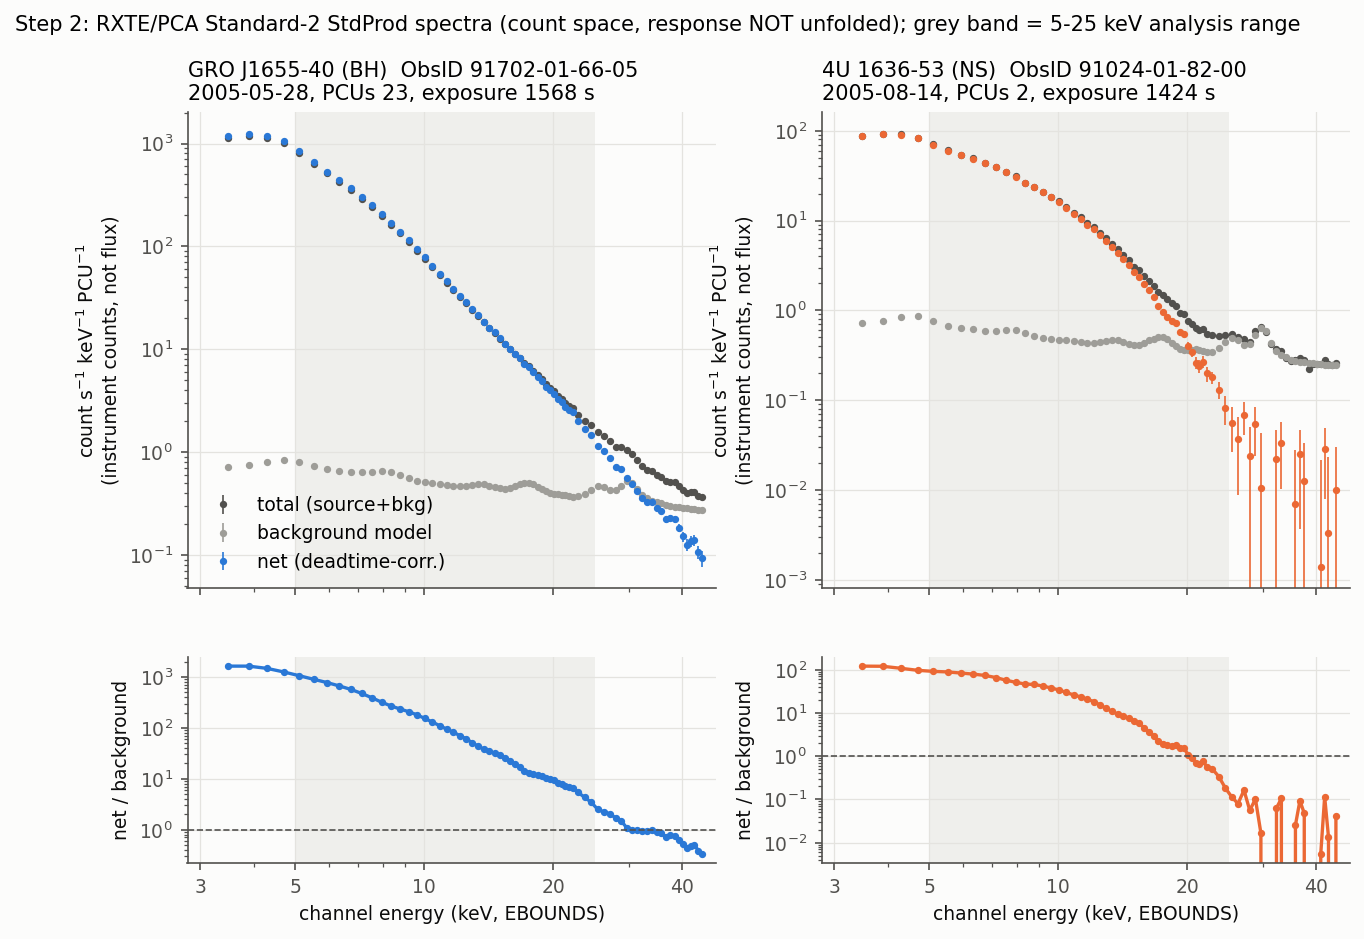
\includegraphics[width=0.92\textwidth]{figures/step2_two_sources.png}
\caption[Two Standard-2 spectra used to validate the data flow]{Data-flow validation on one \BH{} (GRO J1655$-$40,
ObsID 91702-01-66-05) and one \NS{} (4U 1636$-$53, ObsID 91024-01-82-00). Top: total (dark grey), background model
(light grey) and deadtime-corrected net (colour) count rates per keV per PCU against channel energy (EBOUNDS), log--log;
the grey band is the 5--25\,keV analysis range. Bottom: net/background ratio. The point is that the net spectrum is
background-dominated only above $\sim$30\,keV for these bright sources, and that everything is in instrument count space
(no response unfolding). Repo: \file{figures/step2\_two\_sources.png}, script \file{scripts/05\_two\_source\_check.py}.}
\label{fig:step2}
\end{figure}

\subsection{Background subtraction}\label{sec:bkg}
For channel $c$ of observation $i$, with source counts $C^{s}_{c}$ and errors $\sigma^{s}_{c}$, background counts
$C^{b}_{c}$ and errors $\sigma^{b}_{c}$ (function \code{spectra.net\_spectrum}):
\begin{align}
t_s &= \mathtt{EXPOSURE}_s\,\mathtt{AREASCAL}_s, \qquad t_b = \mathtt{EXPOSURE}_b\,\mathtt{AREASCAL}_b,\qquad
\kappa = \mathtt{BACKSCAL}_s/\mathtt{BACKSCAL}_b, \nonumber\\
r^{s}_c &= C^{s}_c/t_s,\quad e^{s}_c = \sigma^{s}_c/t_s,\qquad r^{b}_c = \kappa\,C^{b}_c/t_b,\quad e^{b}_c=\kappa\,\sigma^{b}_c/t_b, \label{eq:srcbkg}\\
r^{\mathrm{net}}_c &= D\,(r^{s}_c - r^{b}_c),\qquad e^{\mathrm{net}}_c = D\,\sqrt{(e^{s}_c)^2 + (e^{b}_c)^2}, \label{eq:net}
\end{align}
in count\,s$^{-1}$ (summed over the PCUs of the spectrum), where $D = 1/(1-\mathrm{DTF})$ is the deadtime correction factor
(\cref{sec:deadtime}). This is the OGIP/XSPEC convention: the same quantity that XSPEC uses after \texttt{data},
\texttt{backgrnd} and \texttt{response}. Non-positive net rates (possible where the source is faint, mainly at
$E>20$\,keV in soft spectra) are kept unchanged: no absolute value, no clipping, no deletion.

\subsection{Deadtime}\label{sec:deadtime}
\textbf{v1 (lower bound).} Only the good-xenon term was available from Standard-2:
\begin{equation}
\mathrm{DTF}^{(\mathrm{v1})} = 10^{-5}\,\mathrm{s}\times \frac{\sum_c C^{s}_c}{t_s\,N_\mathrm{PCU}} ,\label{eq:dtfv1}
\end{equation}
i.e.\ the total (source + background) count rate per PCU times $10\,\mu$s. Median 0.31\% and maximum 6\% in the v1
sample (\file{data/observations.csv}, column \code{dtf\_xe}).
% CHECK: report_v2_zh-TW.md states that the v1 good-xenon median was 0.15%; data/observations.csv (v1) gives 0.31% (matching
% report_zh-TW.md); 0.146% is the median of dtf_xe in the v2 sample (data/v2/observations.csv).

\textbf{v2 onwards (RXTE GOF recipe from Standard-1).} The Standard-1 files of the ObsID are read and the mean rates
inside the spectrum's good time intervals (GTIs) are computed from all 0.125\,s bins whose centre lies in a GTI
(\code{spectra.std1\_rates}): per-PCU good-xenon rates $\mathrm{Xe}_p$ ($p=0,\dots,4$) and array rates $\mathrm{Vp}$
(propane), $\mathrm{Rem}$ (coincident events) and $\mathrm{VLE}$ (very large events). With $N_\mathrm{on}$ the number of
PCUs with $\mathrm{Xe}_p > 1$\,c\,s$^{-1}$ (\code{spectra.std1\_dtf}):
\begin{equation}
\begin{split}
\mathrm{DTF}_p &= 10^{-5}\left(\mathrm{Xe}_p + \frac{\mathrm{Vp}+\mathrm{Rem}}{N_\mathrm{on}}\right) + 6\times10^{-5}\,\frac{\mathrm{VLE}}{N_\mathrm{on}},\\
\mathrm{DTF} &= \frac{1}{|\mathcal P|}\sum_{p\in\mathcal P}\mathrm{DTF}_p,\qquad D = \frac{1}{1-\mathrm{DTF}},
\end{split}\label{eq:dtf}
\end{equation}
with rates in count\,s$^{-1}$ and $\mathcal{P}$ the PCUs of the spectrum. A version with $1.5\times 10^{-4}$\,s per VLE
event (quoted elsewhere on the same GOF page) was stored only as a sensitivity number (\code{dtf\_std1\_vle150us}).
In the v2 sample the Standard-1 coverage of the spectrum GTIs has median 99\% (minimum 88\%), the DTF has median 1.38\% and
maximum 8.8\%; no observation exceeded the 10\% rule. Because $D$ multiplies the whole spectrum, it changes intensities
(representation A) by 1--9\% and leaves shapes (B, H) unchanged.

\subsection{Common energy grid and rebinning}\label{sec:grid}
Gain drifts change the channel-to-energy relation slightly between observations, so every spectrum is rebinned onto one
fixed grid defined by a reference observation (\code{REFERENCE\_OBS = 91702-01-66-05}). Let $\{E^{\mathrm{lo}}_k,
E^{\mathrm{hi}}_k\}$ be the EBOUNDS of the reference response. The grid edges are the union of all EBOUNDS edges between the
edge closest to 5\,keV and the edge closest to 25\,keV:
$e_0 = 4.908$, \dots, $e_{45} = 25.008$\,keV (45 bins, widths 0.41--0.86\,keV; \cref{tab:grid}). For v3b the lower limit
is the edge closest to 3\,keV, giving 50 bins from 2.883\,keV; the 45 bins above 4.908\,keV are identical.
For an observation with its own EBOUNDS, the overlap matrix (\code{spectra.overlap\_matrix})
\begin{equation}
W_{jk} = \frac{\max\!\bigl(0,\ \min(E^{\mathrm{hi}}_k, e_{j+1}) - \max(E^{\mathrm{lo}}_k, e_j)\bigr)}{E^{\mathrm{hi}}_k - E^{\mathrm{lo}}_k}\label{eq:overlap}
\end{equation}
is the fraction of channel $k$ that lies in grid bin $j$ (counts assumed uniform within a channel). The rebinned net
rate per keV per PCU and its error are
\begin{equation}
x_{ij} = \frac{\sum_k W_{jk}\, r^{\mathrm{net}}_{ik}}{N_{\mathrm{PCU},i}\,\Delta e_j},\qquad
\sigma_{ij} = \frac{\sqrt{\sum_k W_{jk}^2\,(e^{\mathrm{net}}_{ik})^2}}{N_{\mathrm{PCU},i}\,\Delta e_j},\qquad \Delta e_j = e_{j+1}-e_j,\label{eq:rebin}
\end{equation}
in count\,s$^{-1}$\,keV$^{-1}$\,PCU$^{-1}$ (array \code{rate} and \code{err} of \file{features.npz}). Division by the
number of PCUs is justified because the effective area grows linearly with the number of PCUs ($\approx 1070$\,cm$^2$ per
PCU at 6\,keV). The error formula treats channels as independent; two grid bins that share one channel are therefore
weakly correlated, which is ignored. The total (source + background) and background spectra are rebinned in the same
way (\code{srate}, \code{brate}). The gain drift within epoch~5 is at most 0.85 channel (median 0.17) relative to the
reference.

\begin{table}[htbp]
\centering\scriptsize
\caption[The common energy grid]{The 45-bin common energy grid (keV), from the EBOUNDS of observation 91702-01-66-05
(\file{data/v2/processed/features.npz}, key \code{edges}; identical in every RXTE sample). Bin $j$ spans $[e_j,e_{j+1})$.
The v3b grid adds five bins below: 2.883, 3.287, 3.691, 4.096, 4.502, 4.908\,keV.}
\label{tab:grid}
\setlength{\tabcolsep}{3pt}
\begin{tabular}{@{}rr@{\hspace{10pt}}rr@{\hspace{10pt}}rr@{\hspace{10pt}}rr@{\hspace{10pt}}rr@{}}
\toprule
$j$ & $e_j$ & $j$ & $e_j$ & $j$ & $e_j$ & $j$ & $e_j$ & $j$ & $e_j$\\
\midrule
0 & 4.908 & 10 & 9.001 & 20 & 13.149 & 30 & 17.346 & 40 & 21.588 \\
1 & 5.315 & 11 & 9.414 & 21 & 13.566 & 31 & 17.768 & 41 & 22.014 \\
2 & 5.722 & 12 & 9.827 & 22 & 13.985 & 32 & 18.191 & 42 & 22.441 \\
3 & 6.130 & 13 & 10.240 & 23 & 14.403 & 33 & 18.614 & 43 & 23.295 \\
4 & 6.538 & 14 & 10.654 & 24 & 14.822 & 34 & 19.038 & 44 & 24.151 \\
5 & 6.948 & 15 & 11.069 & 25 & 15.242 & 35 & 19.462 & 45 & 25.008 \\
6 & 7.357 & 16 & 11.484 & 26 & 15.662 & 36 & 19.886 & & \\
7 & 7.767 & 17 & 11.899 & 27 & 16.082 & 37 & 20.311 & & \\
8 & 8.178 & 18 & 12.315 & 28 & 16.503 & 38 & 20.736 & & \\
9 & 8.589 & 19 & 12.732 & 29 & 16.924 & 39 & 21.162 & & \\
\bottomrule
\end{tabular}
\end{table}

\subsection{Summary quantities, errors and quality rules}\label{sec:quality}
For each observation (\file{04\_fetch\_process.py}):
\begin{align}
F_i &= \sum_{j=0}^{44} x_{ij}\Delta e_j \quad[\mathrm{count\,s^{-1}\,PCU^{-1}}],\qquad
\sigma_{F,i} = \Bigl(\sum_j (\sigma_{ij}\Delta e_j)^2\Bigr)^{1/2},\qquad \mathrm{S/N}_i = F_i/\sigma_{F,i}, \label{eq:F}\\
f^{\mathrm{bkg}}_i &= \frac{\sum_j x^{b}_{ij}\Delta e_j}{\sum_j x^{s}_{ij}\Delta e_j}\quad\text{(background fraction, 5--25 keV)}.\nonumber
\end{align}
An observation is accepted only if all of the following hold (otherwise the next candidate of the same time group is
tried): all files present and readable, 129 channels, EBOUNDS cover 5--25\,keV; spectrum exposure $\ge 1000$\,s;
$\mathrm{S/N}\ge 10$; $\mathrm{DTF}\le 0.10$; header position \texttt{RA\_OBJ/DEC\_OBJ} within 0.1$^\circ$ of the
source position; all values finite. $F_i>0$ is guaranteed by the S/N rule, so the shape normalisation
(\cref{eq:B}) is always defined.

\subsection{Response check and response-normalised spectra}\label{sec:pl2}
A fixed photon spectrum $N(E)=E^{-2}$ (photon index $\Gamma=2$, no absorption, normalised to
1\,ph\,cm$^{-2}$\,s$^{-1}$\,keV$^{-1}$ at 1\,keV) is folded through each observation's response matrix $R(E,c)$ (\code{spectra.powerlaw\_folded}) and rebinned
like the data:
\begin{equation}
P_{ic} = \sum_{\ell} R_i(E_\ell,c)\int_{E^{\mathrm{lo}}_\ell}^{E^{\mathrm{hi}}_\ell} E^{-2}\,dE,\qquad
p_{ij} = \frac{\sum_c W_{jc}P_{ic}}{N_{\mathrm{PCU},i}\,\Delta e_j}\quad(\text{key \code{pl2}}).\label{eq:pl2}
\end{equation}
The across-observation scatter of $p_{ij}/\median_i p_{ij}$ measures how much the instrument response alone changes the
count spectrum: median 3.7\%, maximum 11--12.7\%, driven by the PCU combination (\cref{fig:response}). BH and NS have
similar PCU-combination mixtures (mean tilt 2.0\% vs 2.4\% in v1), so this is treated as noise rather than as a class
shortcut. From v4b2 on, $p_{ij}$ also defines the response-normalised representations R and H$_R$ (\cref{sec:reps}),
which can be compared across gain epochs.

\begin{figure}[htbp]
\centering
\begin{subfigure}{0.49\textwidth}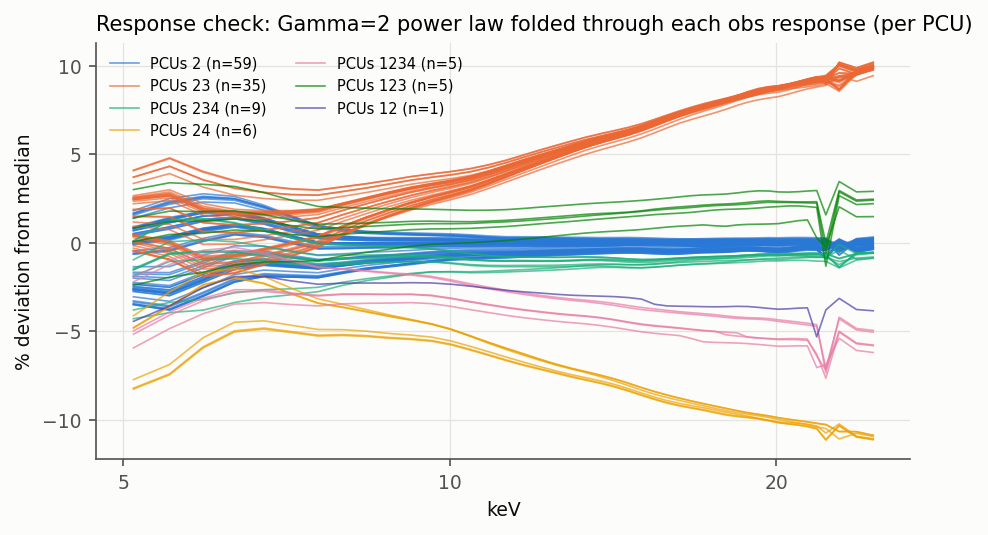
\includegraphics[width=\textwidth]{figures/step3_response_variation.png}\caption{v1 (120 observations)}\end{subfigure}
\begin{subfigure}{0.49\textwidth}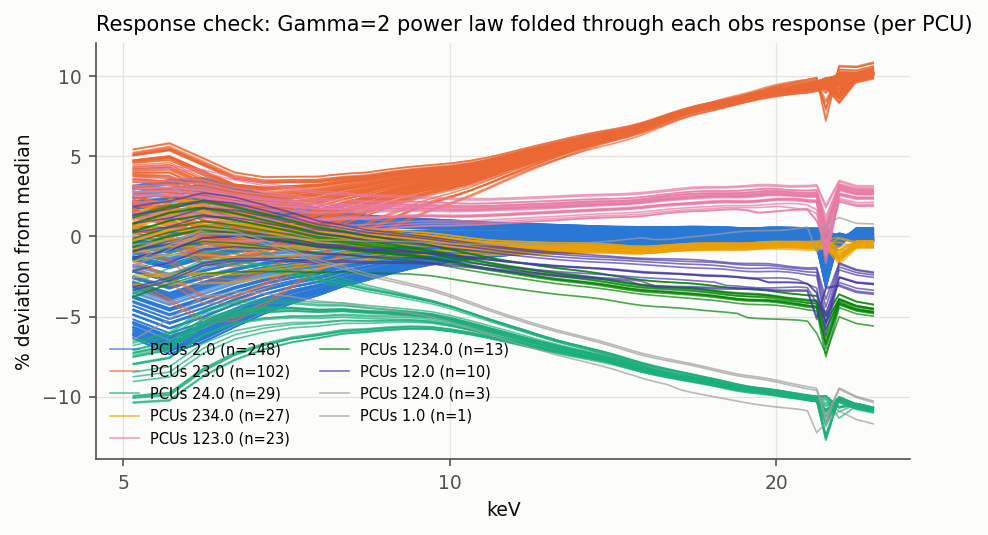
\includegraphics[width=\textwidth]{figures/v2/step3_response_variation.png}\caption{v2 (456 observations)}\end{subfigure}
\caption[Response variation between observations]{Response check: a fixed $\Gamma=2$ power law folded through each
observation's response, per PCU, shown as percentage deviation from the median over observations, against energy;
colour = PCU combination. The spread (a few per cent, up to $\sim$10\% at 25\,keV) is set by which PCUs were on, not by the
source class. Repo: \file{figures/step3\_response\_variation.png}, \file{figures/v2/step3\_response\_variation.png};
script \file{scripts/06\_dataset\_checks.py}.}
\label{fig:response}
\end{figure}

\subsection{Independent check with XSPEC}\label{sec:xspec}
For 12 randomly chosen v2 observations (seed 42; 10 sources; net rates 5--950\,c\,s$^{-1}$), HEASoft~6.37.1/XSPEC
(\texttt{data}, \texttt{backgrnd}, \texttt{response}, \texttt{ignore **-5.0 25.0-**}, \texttt{tclout rate}) and
\cref{eq:net} with $D=1$ summed over the same noticed channels (10--52 or 10--53) agree to $3\times10^{-10}$ (rate) and
$4\times10^{-10}$ (error) relative (\file{results/v2/xspec\_crosscheck.csv}, \file{scripts/10\_xspec\_crosscheck.py}). This
validates \cref{eq:srcbkg,eq:net}; it does not validate the deadtime, the rebinning, or the background model itself.

% -----------------------------------------------------------------------------------------------------
\section{Spectral representations}\label{sec:reps}
% -----------------------------------------------------------------------------------------------------

All representations are computed per observation from the rebinned spectrum $x_{i\cdot}$; none uses information from
other observations (the training-set standardisation of \cref{sec:scaler} is a separate step inside the model).
Code: \file{07\_train\_eval.py}, \code{v3lib.v2\_representations}, \file{12\_v3b\_extended\_band.py},
\code{reps\_R} in \file{22\_v4b2\_analysis.py}.

\paragraph{A (intensity kept).} With scale $a = 0.1$\,count\,s$^{-1}$\,keV$^{-1}$\,PCU$^{-1}$ (\code{ASINH\_SCALE}),
\begin{equation}
A_{ij} = \operatorname{asinh}\!\left(x_{ij}/a\right),\qquad j=0,\dots,44. \label{eq:A}
\end{equation}
$\operatorname{asinh}(u)\approx \sgn(u)\ln(2|u|)$ for $|u|\gg1$ and $\approx u$ near 0, so A is log-like for bright bins
and defined for the (rare) negative bins. A keeps the absolute count rate, which depends on distance, absorption and
accretion rate as well as on the compact object.

\paragraph{B (shape).}
\begin{equation}
B_{ij} = x_{ij}/F_i\quad[\mathrm{keV^{-1}}],\qquad \textstyle\sum_j B_{ij}\Delta e_j = 1. \label{eq:B}
\end{equation}

\paragraph{H (two count-space colours).} Four bands are formed from the grid bins whose geometric centre
$\bar e_j=\sqrt{e_je_{j+1}}$ lies in a nominal interval (\code{v3lib.band}); the exact bin ranges are in \cref{tab:bands}:
\begin{equation}
C_{i,m} = \sum_{j\in b_m} x_{ij}\Delta e_j\ \ [\mathrm{count\,s^{-1}\,PCU^{-1}}],\qquad
\vect{h}_i = (h_{i1},h_{i2}) = \left(\frac{C_{i,2}}{C_{i,1}},\ \frac{C_{i,4}}{C_{i,3}}\right). \label{eq:H}
\end{equation}
$h_1$ (``soft colour'', $\approx$\,7--10 over 5--7\,keV) and $h_2$ (``hard colour'', $\approx$\,16--25 over 10--16\,keV) are
linear ratios. The pre-registration originally specified $\log_{10}$ colours; before any v2 model was trained, two BH
spectra (95409-01-29-00 GX\,339$-$4, 60113-01-34-00 XTE J1650$-$500) were found with a slightly negative 16--25\,keV net
sum, so the linear ratio was adopted (logged in \file{reports/decision\_log.md}). Denominators $C_1, C_3$ are positive
for every observation (asserted in the code); numerators may be $\le 0$ and are kept.

\paragraph{HI, H+B, HI+A.} $\mathrm{HI}_i = (h_{i1},h_{i2},\log_{10}F_i)$; $\mathrm{H{+}B}_i = (\vect{h}_i, B_{i0},\dots,B_{i44})$
(47 features); $\mathrm{HI{+}A}_i = (\mathrm{HI}_i, A_{i0},\dots,A_{i44})$ (48 features).

\paragraph{v3b (3--25\,keV).} On the 50-bin grid: $F^{(3)}_i=\sum_{j}x_{ij}\Delta e_j$ over all 50 bins;
$\mathrm{B3}_{ij} = x_{ij}/F^{(3)}_i$; $\mathrm{H3}_i = (C_{i,0}/C_{i,1},\ C_{i,2}/C_{i,1},\ C_{i,4}/C_{i,3})$ where
$C_{i,0}$ sums the five bins with centre in $[2.8,5)$\,keV (2.883--4.908\,keV). The soft colour has 3--5\,keV in the
numerator and a denominator that is always positive.

\paragraph{R and H$_R$ (response-normalised; v4b2 onwards).} With $p_{ij}$ of \cref{eq:pl2}:
\begin{equation}
R_{ij} = \frac{x_{ij}}{p_{ij}},\qquad P_{i,m} = \sum_{j\in b_m}p_{ij}\Delta e_j,\qquad
\vect{h}^{R}_i = \left(\frac{C_{i,2}/P_{i,2}}{C_{i,1}/P_{i,1}},\ \frac{C_{i,4}/P_{i,4}}{C_{i,3}/P_{i,3}}\right). \label{eq:HR}
\end{equation}
H$_R$ is the colour of the data relative to the colour a $\Gamma=2$ power law would have through the same response; it
removes first-order response differences (e.g.\ between gain epochs). Its predictions agree with H at Spearman 0.994
(\cref{ch:phase2}).

\begin{table}[htbp]
\centering\small
\caption[Colour bands]{The four colour bands of H (and H$_R$): grid bins whose geometric centre lies in the nominal
interval, and the actual energy range they cover (computed from \code{edges}).}
\label{tab:bands}
\begin{tabular}{@{}llccc@{}}
\toprule
Band & nominal interval (centre rule) & bins $j$ & $n$ bins & actual range [keV] \\
\midrule
$b_1$ & $[5,7)$ & 0--4 & 5 & 4.908--6.948 \\
$b_2$ & $[7,10)$ & 5--11 & 7 & 6.948--9.827 \\
$b_3$ & $[10,16)$ & 12--26 & 15 & 9.827--16.082 \\
$b_4$ & $[16,25.1)$ & 27--44 & 18 & 16.082--25.008 \\
$b_0$ (v3b) & $[2.8,5)$ & 5 bins of the 50-bin grid & 5 & 2.883--4.908 \\
\bottomrule
\end{tabular}
\end{table}

\Cref{fig:meanspectra} shows the class-averaged spectra in the A, B and H representations.

\begin{figure}[htbp]
\centering
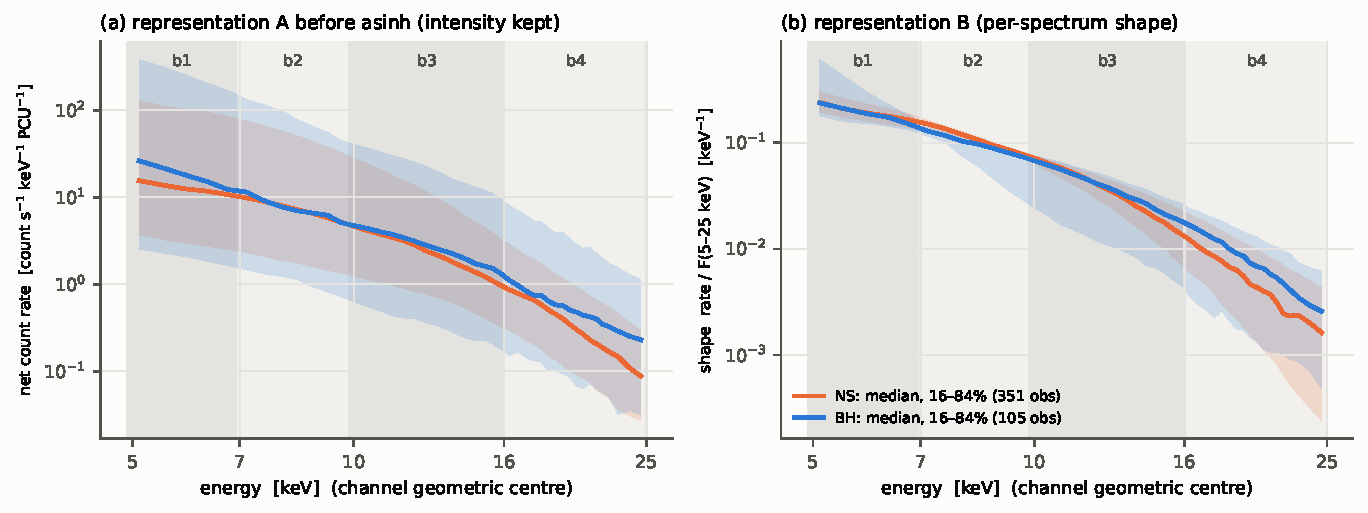
\includegraphics[width=\textwidth]{figures/generated/G2_mean_spectra.pdf}
\caption[Count-space spectra of BHs and NSs with the colour bands]{Median (line) and 16--84\% range (shading) of the
v2 count-space spectra, BH (blue, 105 observations) and NS (orange, 351 observations). (a) net rate per keV per PCU
(the quantity transformed by asinh in representation A); (b) per-spectrum shape B. Grey and light bands mark the four
colour bands $b_1$--$b_4$ of \cref{tab:bands}. Non-positive bins are omitted from the percentiles. The class medians
differ mainly in the overall slope above 10\,keV and overlap strongly, which is why two colours capture most of the
shape information (\cref{ch:phase1}). Generated for this report from \file{data/v2/processed/features.npz}
(\file{report\_en/figures/generated/make\_figures.py}).}
\label{fig:meanspectra}
\end{figure}

% -----------------------------------------------------------------------------------------------------
\section{HEXTE high-energy colours (v4b3)}\label{sec:hexte}
% -----------------------------------------------------------------------------------------------------

Only HEXTE cluster~B is used (\file{19\_v4b3\_hexte.py}), because it rocked between source and background until
2009-12-14 16:10\,UT (MJD 55179.6736); observations on or after that date, or without cluster-B files, have no HEXTE
features (60 of the 456 v2 observations). Header keyword \texttt{DEADAPP = T} (deadtime already applied) is required.
The net cluster-B spectrum follows \cref{eq:srcbkg,eq:net} with $D=1$; band rates $F_X(25\text{--}40)$ and
$F_X(40\text{--}60)$ (count\,s$^{-1}$ per cluster) use the overlap matrix of \cref{eq:overlap} on the RMF EBOUNDS. With
$F_\mathrm{PCA}(16\text{--}25)=C_{i,4}$ of \cref{eq:H}:
\begin{equation}
X_1 = \frac{F_X(25\text{--}40)}{F_\mathrm{PCA}(16\text{--}25)},\qquad X_2 = \frac{F_X(40\text{--}60)}{F_X(25\text{--}40)} .\label{eq:hexte}
\end{equation}
$X_1$ is a cross-instrument count ratio and is only used as a feature. A colour is set to missing when its denominator
has S/N $<3$ ($X_1$: 3 observations; $X_2$: 144, of which 23 BH). Missing colours are filled with the training-fold
median, and one 0/1 indicator per colour is appended (inside the LOSO loop; \code{hx\_features}); H+X therefore has 6
columns.

% -----------------------------------------------------------------------------------------------------
\section{Type-I X-ray bursts}\label{sec:bursts}
% -----------------------------------------------------------------------------------------------------

Type-I bursts are seconds-long thermonuclear flashes that only NSs produce; an observation containing one carries a
label shortcut and a distorted spectrum. Three procedures are used.

\paragraph{Standard-1 burst detector (v4; \file{17\_v4\_burst\_detect.py}).} The 1\,s light curve $r(t)$ is the sum of
good-xenon counts of the spectrum's PCUs over complete 1\,s bins inside the GTIs. With $\mu,s$ the mean and standard
deviation of all bins: candidates are bins with $r>\mu+4s$; candidates closer than 30\,s are merged into one event. For
an event with peak $r_\mathrm{pk}$ at $t_\mathrm{pk}$ and persistent level $r_0$ (median of the 60\,s before the event, or
of the whole curve if fewer than 60 bins), amplitude $A=r_\mathrm{pk}-r_0$ and levels $L_q = r_0+qA$:
\begin{equation}
\text{burst} \iff r_\mathrm{pk}\ge 1.5\,r_0\ \wedge\ t_\mathrm{rise}\le 10\,\mathrm{s}\ \wedge\ 3\le t_{1/2}\le 300\,\mathrm{s}\ \wedge\ n_{25}\ge 3,\label{eq:burst}
\end{equation}
where $t_\mathrm{rise} = t_\mathrm{pk} - \max\{t<t_\mathrm{pk}: r(t)<L_{0.25}\}$,
$t_{1/2} = \min\{t>t_\mathrm{pk}: r(t)<L_{0.5}\} - t_\mathrm{pk}$, and $n_{25}$ is the number of contiguous 1\,s bins around
the peak above $L_{0.25}$. The burst interval runs from the last time before the peak below $L_{0.25}$ to the first time
after it below $L_{0.1}$. Thresholds are \code{V4\_BURST} in \file{config.py}, following the search criterion of
\citet{Galloway2008}. Every candidate was also inspected by eye (\file{results/v4/burst\_visual.csv}).

\paragraph{MINBAR matching (v7b1; \code{v7lib.load\_minbar}, \code{gti\_utc}, \code{minbar\_flag}).} The spectrum GTIs
(\texttt{STDGTI}, mission elapsed time in TT) are converted to MJD(TT) $=\mathtt{MJDREF}+t/86400$ and then to UTC with
\texttt{astropy} (TT$-$UTC $=64.18$\,s; round-trip error $<1$\,ms). A MINBAR burst occupies $[T,\,T+\mathrm{dur}]$
(dur missing $\Rightarrow$ 300\,s). Primary rule: an observation is contaminated if a burst interval overlaps a GTI
\emph{and} the burst has the same ObsID or originates within 1$^\circ$ (PCA field of view) of the source. The literal
pre-registered rule (any burst from any origin) is kept as a sensitivity set.

\paragraph{NICER burst rule (v9--v13; \code{v9lib.burst\_events}).} The same \cref{eq:burst} is applied to the
2--10\,keV 1\,s light curve built from events inside the good intervals (\cref{sec:nicer}); every 128\,s segment that
overlaps $[t_\mathrm{start}-20\,\mathrm{s},\,t_\mathrm{end}+200\,\mathrm{s}]$ of an automatically detected burst is removed.

% -----------------------------------------------------------------------------------------------------
\section{Low-frequency timing from RXTE Standard-1 (v5--v10)}\label{sec:std1timing}
% -----------------------------------------------------------------------------------------------------

\Cref{fig:timingpipeline} summarises the chain from light curve to features; this section gives the formulae.

\begin{figure}[htbp]
\centering
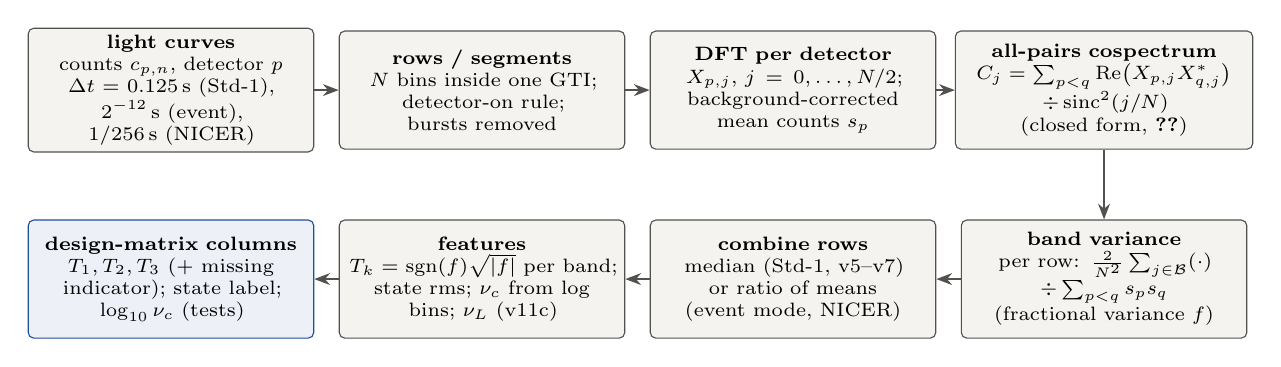
\begin{tikzpicture}[every node/.style={font=\scriptsize},
  box/.style={draw=inkgrey, rounded corners=2pt, fill=boxgrey, align=center, minimum height=15mm, text width=3.45cm, inner sep=2.5pt, execute at begin node={\hyphenpenalty=10000\relax}},
  outbox/.style={box, fill=tagprim!8, draw=tagprim},
  arr/.style={-{Stealth[length=2mm]}, thick, inkgrey}]
% row 1: left to right
\node[box] (lc)    at (0,0)    {\textbf{light curves}\\ counts $c_{p,n}$, detector $p$\\ $\Delta t$ = 0.125\,s (Std-1),\\ $2^{-12}$\,s (event),\\ $1/256$\,s (NICER)};
\node[box] (seg)   at (3.95,0) {\textbf{rows / segments}\\ $N$ bins inside one GTI;\\ detector-on rule;\\ bursts removed};
\node[box] (fft)   at (7.9,0)  {\textbf{DFT per detector}\\ $X_{p,j}$, $j=0,\dots,N/2$;\\ background-corrected\\ mean counts $s_p$};
\node[box, text width=3.6cm] (cross) at (11.85,0){\textbf{all-pairs cospectrum}\\ \mbox{$C_j=\sum_{p<q}\Real\bigl(X_{p,j}X^{*}_{q,j}\bigr)$}\\ $\div\,\mathrm{sinc}^2(j/N)$\\ (closed form, \cref{eq:allpairs})};
% row 2: right to left
\node[box] (band)  at (11.85,-2.4) {\textbf{band variance}\\ per row: $\frac{2}{N^2}\sum_{j\in\mathcal B}(\cdot)$\\ $\div\sum_{p<q}s_ps_q$\\ (fractional variance $f$)};
\node[box] (agg)   at (7.9,-2.4)   {\textbf{combine rows}\\ median (Std-1, v5--v7)\\ or ratio of means\\ (event mode, NICER)};
\node[box] (feat)  at (3.95,-2.4)  {\textbf{features}\\ $T_k=\sgn(f)\sqrt{|f|}$ per band;\\ state rms; $\nu_c$ from log\\ bins; $\nu_L$ (v11c)};
\node[outbox] (dm)    at (0,-2.4)     {\textbf{design-matrix columns}\\ $T_1,T_2,T_3$ (+ missing\\ indicator); state label;\\ $\log_{10}\nu_c$ (tests)};
\draw[arr] (lc)--(seg); \draw[arr] (seg)--(fft); \draw[arr] (fft)--(cross); \draw[arr] (cross)--(band);
\draw[arr] (band)--(agg); \draw[arr] (agg)--(feat); \draw[arr] (feat)--(dm);
\end{tikzpicture}
\caption[Timing-feature pipeline]{Timing-feature pipeline shared by RXTE Standard-1 (v5--v10), RXTE event mode (v8c) and
NICER (v9--v13). Differences between the instruments are in the bin width, the segment length, the ``detector'' (PCU or
NICER MPU), whether rows are combined by the median or by the ratio of means, and the frequency bands
(\cref{tab:timingbands}). Drawn for this report.}
\label{fig:timingpipeline}
\end{figure}

\subsection{Rows, detectors and background}
A Standard-1 file stores, for each 128\,s row, $N=1024$ counts per PCU in $\Delta t = 0.125$\,s bins. Only rows lying
completely inside a spectrum GTI are used (start $\ge$ GTI start $-1$\,ms and end $\le$ GTI stop $+1$\,ms;
\code{v5lib.std1\_rows}). PCU $p$ is \emph{on} in a row if each of the eight 128-bin blocks (16\,s) has at least one count
(\code{v5lib.pcus\_on}). The background count rate per PCU is taken from the Standard-2 background spectrum over all
channels, $b = \sum_c C^b_c/(t_b N_{\mathrm{PCU},b})$ count\,s$^{-1}$ (assumed equal for all PCUs). For a detector group
or a single PCU with counts $c_n$ and $n_\mathrm{det}$ detectors, the mean \emph{source} counts per bin is
$s = \bar c - n_\mathrm{det}\, b\,\Delta t$; a row is invalid if any $s\le0$.

\subsection{Fourier conventions and the binning correction}
The discrete Fourier transform is $X_j = \sum_{n=0}^{N-1} c_n e^{-2\pi i jn/N}$, $j=0,\dots,N/2$ (\code{numpy.fft.rfft}),
frequency $\nu_j = j/(N\Delta t)$ (for 128\,s rows, $\nu_j = j/128$\,Hz). Parseval's relation gives
$\frac{1}{N}\sum_n (c_n-\bar c)^2 = \frac{1}{N^2}\sum_{j\ne0}|X_j|^2 \approx \frac{2}{N^2}\sum_{j=1}^{N/2}|X_j|^2$,
so $\frac{2}{N^2}\sum_{j\in\mathcal B}|X_j|^2$ is the variance (in counts$^2$ per bin$^2$) contributed by band
$\mathcal B$. Integrating counts over bins of width $\Delta t$ multiplies the Fourier amplitude by
$\sinc(j/N) = \sin(\pi j/N)/(\pi j/N)$ \citep[Eq.~2.19]{vanderKlis1989}; every power is divided by $\sinc^2(j/N)$.

\subsection{Two-group cospectrum (v5)}\label{sec:v5timing}
The PCUs that are on are sorted; those in even positions form group A, those in odd positions group B (at least two
PCUs are required). With $x_n,y_n$ the summed counts of the groups, $X_j,Y_j$ their transforms, and $s_x,s_y$ their
background-corrected mean source counts per bin (\code{v5lib.row\_features}):
\begin{equation}
V_\mathcal{B} = \frac{2}{N^2}\sum_{j\in\mathcal B}\frac{\Real(X_jY_j^{*})}{\sinc^2(j/N)},\qquad f_\mathcal{B} = \frac{V_\mathcal{B}}{s_x s_y} .\label{eq:v5cross}
\end{equation}
Because the Poisson (and deadtime) noise of different detectors is uncorrelated, the expected value of the cospectrum
$\Real(X_jY_j^*)$ in the absence of source variability is zero \citep{Bachetti2015,BachettiHuppenkothen2018}; no Poisson
level has to be modelled. $f_\mathcal{B}$ is the fractional variance (rms$^2$ normalised to the source mean) in band
$\mathcal B$. Per observation, the \emph{median} over valid rows is taken (robust to rare rows with flares or bursts);
fewer than 3 valid rows $\Rightarrow$ missing. Features are signed square roots,
\begin{equation}
\begin{split}
T_k &= \sgn\!\bigl(\median_r f_{k,r}\bigr)\sqrt{\bigl|\median_r f_{k,r}\bigr|},\qquad k\in\{1,2,3\},\\
T_\mathrm{tot} &= \sgn(F)\sqrt{|F|},\qquad F=\textstyle\sum_k \median_r f_{k,r},
\end{split}\label{eq:signedsqrt}
\end{equation}
(fractional rms, which may be slightly negative because of noise). The bands are listed in \cref{tab:timingbands}.
As an implementation check the conventional auto-power estimator $(|Z_j|^2 - N\bar z)/\sinc^2(j/N)$ of $z=x+y$
(Poisson level $N\bar z$, no deadtime) was also computed; for 276 S1 observations with 20--500 source c\,s$^{-1}$\,PCU$^{-1}$
the two versions of $T_2$ agree at Spearman 0.970.

\subsection{All-pairs estimator and single-PCU hybrid (v6)}\label{sec:allpairs}
Using every pair of the $n$ PCUs that are on, rather than one A/B split, reduces the noise (\code{v6lib.allpairs\_row}).
With per-PCU transforms $X_{p,j}$ and source means $s_p$:
\begin{equation}
\sum_{p<q}\Real(X_{p,j}X_{q,j}^*) = \frac{\bigl|\sum_p X_{p,j}\bigr|^2-\sum_p|X_{p,j}|^2}{2},\qquad
f_\mathcal{B} = \frac{\frac{2}{N^2}\sum_{j\in\mathcal B}\frac{|\sum_pX_{p,j}|^2-\sum_p|X_{p,j}|^2}{2\sinc^2(j/N)}}{\frac{(\sum_p s_p)^2-\sum_p s_p^2}{2}} .\label{eq:allpairs}
\end{equation}
Rows with a single PCU on use the auto-power estimator $f_\mathcal{B} = \frac{2}{N^2}\sum_{j\in\mathcal B}
\frac{|X_j|^2-N\bar c}{\sinc^2(j/N)}\big/ s^2$, but only if the total count rate is $\le 500$\,c\,s$^{-1}$ (where the
deadtime-free Poisson level is adequate); otherwise the row is invalid. $T_k^\ast$ is the signed square root of the
median over all valid rows (pair rows and single rows together). In synthetic tests the noise variance drops by 31\%,
33\% and 41\% for 3, 4 and 5 PCUs (theory 33\%, 33\%, 40\%) without bias; missing values over 8\,350 observations fall from
942 to 341.

\subsection{Characteristic frequency $\nu_c$ (v6)}\label{sec:nuc}
Nine logarithmic Fourier-index bins are formed from $\mathrm{unique}(\mathrm{round}(\mathrm{geomspace}(1,512,10)))$
$=\{1,2,4,8,\dots,512\}$ as $[1,1],[2,3],[4,7],\dots,[256,511]$ (\cref{tab:nucbins}). For each bin $b$, $P_b$ is the
median over rows of the fractional variance (\cref{eq:allpairs}) in that bin; the bin centre is
$\nu_b=\sqrt{j_\mathrm{lo}j_\mathrm{hi}}/128$\,Hz and its width in $\ln\nu$ is
$\Delta_b = \ln\bigl((j_\mathrm{hi}+0.5)/(j_\mathrm{lo}-0.5)\bigr)$. The $\nu P_\nu$ centroid is (\code{v6lib.nu\_centroid})
\begin{equation}
\ln\nu_c = \frac{\sum_b w_b\ln\nu_b}{\sum_b w_b},\qquad w_b = \frac{\max(P_b,0)}{\Delta_b},\label{eq:nuc}
\end{equation}
missing if $T^\ast_\mathrm{tot}<0.05$ or $\sum_b w_b\le0$. Since $P_b/\Delta_b$ is the power per unit $\ln\nu$ (i.e.\
$\nu P_\nu$), $\nu_c$ is the frequency around which most of the variability power per logarithmic frequency interval lies:
a model-free proxy for a break or characteristic frequency. Synthetic sinusoids at 0.05, 0.5 and 3\,Hz are recovered
within one log bin.

\begin{table}[htbp]
\centering\small
\caption[Timing frequency bands]{Fourier-index bands and their frequencies. Standard-1 and NICER use 128\,s rows or
segments ($\nu_j=j/128$\,Hz); RXTE event mode uses 16\,s segments ($\nu_j=j/16$\,Hz). From \file{config.py}.}
\label{tab:timingbands}
\begin{tabular}{@{}lllll@{}}
\toprule
Band & index $j$ & frequency [Hz] & data & config name \\
\midrule
$T_1$ & 2--12 & 0.0156--0.094 & Std-1, NICER & \code{V5\_BANDS\_J}, \code{V9\_T\_BANDS\_J} \\
$T_2$ & 13--128 & 0.102--1.000 & Std-1, NICER & \\
$T_3$ & 129--511 & 1.008--3.992 & Std-1, NICER & \\
state (v7a) & 13--511 & 0.102--3.992 & Std-1 & \code{V7\_RMS\_J} \\
state (v9+) & 13--1280 & 0.102--10.0 & NICER & \code{V9\_STATE\_J} \\
white monitor & 12288--16383 & 96--128 & NICER & \code{V9\_WHITE\_J} \\
LC & 16--63 & 1.0--3.94 & event mode & \code{V8\_HF\_BANDS\_J} \\
HF1 & 64--1023 & 4.0--63.9 & event mode & \\
HF2 & 1024--8191 & 64--512 & event mode & \\
HF3 & 8192--16383 & 512--1024 & event mode & \\
NULL & 24576--32767 & 1536--2048 & event mode & \\
\bottomrule
\end{tabular}
\end{table}

\begin{table}[htbp]
\centering\small
\caption[Bins of the $\nu P_\nu$ centroid]{Bins of the $\nu P_\nu$ centroid. Left: RXTE Standard-1 (v6; 9 bins, $\nu_b$ and
$\Delta_b$ of \cref{eq:nuc}). Right: NICER (v9--v13; 13 octave bins $j\in[2^k,2^{k+1}-1]$, centre $2^{k+0.5}/128$\,Hz).
Computed from the code (\file{v6lib.py}, \file{v9lib.py}).}
\label{tab:nucbins}
\begin{tabular}{@{}rrrr@{\hspace{18pt}}rrr@{}}
\toprule
\multicolumn{4}{c}{Standard-1 (v6)} & \multicolumn{3}{c}{NICER (v9+)}\\
\cmidrule(r){1-4}\cmidrule(l){5-7}
$[j_\mathrm{lo},j_\mathrm{hi}]$ & $\nu_b$ [Hz] & range [Hz] & $\Delta_b$ & $k$ & $[j_\mathrm{lo},j_\mathrm{hi}]$ & $\nu_k$ [Hz]\\
\midrule
$[1,1]$ & 0.0078 & 0.0039--0.0117 & 1.099 & 0 & $[1,1]$ & 0.011 \\
$[2,3]$ & 0.0191 & 0.0117--0.0273 & 0.847 & 1 & $[2,3]$ & 0.022 \\
$[4,7]$ & 0.0413 & 0.0273--0.0586 & 0.762 & 2 & $[4,7]$ & 0.044 \\
$[8,15]$ & 0.0856 & 0.0586--0.121 & 0.726 & 3 & $[8,15]$ & 0.088 \\
$[16,31]$ & 0.174 & 0.121--0.246 & 0.709 & 4 & $[16,31]$ & 0.177 \\
$[32,63]$ & 0.351 & 0.246--0.496 & 0.701 & 5 & $[32,63]$ & 0.354 \\
$[64,127]$ & 0.704 & 0.496--0.996 & 0.697 & 6 & $[64,127]$ & 0.707 \\
$[128,255]$ & 1.411 & 0.996--1.996 & 0.695 & 7 & $[128,255]$ & 1.414 \\
$[256,511]$ & 2.826 & 1.996--3.996 & 0.694 & 8 & $[256,511]$ & 2.828 \\
 & & & & 9--12 & $[512,1023]$--$[4096,8191]$ & 5.66, 11.3, 22.6, 45.3 \\
\bottomrule
\end{tabular}
\end{table}

\subsection{State index (v7a)}\label{sec:state}
The variability state of an observation is classified by its fractional rms in 0.1--4\,Hz ($j=13$--511), computed with
\cref{eq:allpairs} from rows with $\ge2$ PCUs only (no single-PCU rows, because their Poisson level would need a deadtime
model), after removing every row that overlaps a burst interval $[t_\mathrm{start}-20\,\mathrm{s},\ \text{end}]$ (MINBAR
field-of-view rule and the v4 detector; \code{v7lib.state\_rms}). With $\rho = \sgn(\median_r f)\sqrt{|\median_r f|}$:
\begin{equation}
\text{state} = \begin{cases}\text{hard-like} & \rho>0.10\\ \text{soft-like} & \rho<0.075\\ \text{intermediate} & \text{otherwise}\end{cases}
\qquad(\text{unknown if fewer than 3 rows}),\label{eq:state}
\end{equation}
the thresholds of \citet[Table 2]{RemillardMcClintock2006}, which are defined for 0.1--10\,Hz; the 4\,Hz Nyquist limit
of Standard-1 makes $\rho$ slightly low and the hard-like class conservative. NICER (v9 onwards) uses the full
0.1--10\,Hz band. ``Soft-like/hard-like'' are operational variability classes, not full spectral-state assignments.

% -----------------------------------------------------------------------------------------------------
\section{High-frequency timing from RXTE event mode (v8c)}\label{sec:eventmode}
% -----------------------------------------------------------------------------------------------------

An event file qualifies if \texttt{DATAMODE} matches \texttt{\^{}E\_\textbackslash d+us\_\textbackslash d+M\_0\_\textbackslash d+s\$},
\texttt{TDDES2} contains the six anode chains \texttt{X1L\^{}X1R\^{}X2L\^{}X2R\^{}X3L\^{}X3R}, \texttt{TIMEDEL}~$\le2^{-12}$\,s and a
\texttt{PCUID} column exists (\code{v8lib.mode\_qualifies}); if several modes qualify, the one with the largest total size
is used. Events are binned at $\Delta t=2^{-12}$\,s (Nyquist 2048\,Hz) in 16\,s segments ($N=65536$) lying completely in
(spectrum GTI) $\cap$ (event-file GTI) and not overlapping a burst interval. A PCU is on if each of the 16 one-second
sub-intervals has an event; $\ge2$ PCUs are required. For segment $r$, with \cref{eq:allpairs},
$\mathrm{num}_{\mathcal B,r} = \frac{2}{N^2}\sum_{j\in\mathcal B}\mathrm{cross}_j$ and
$\mathrm{den}_r=\sum_{p<q}s_ps_q$. The pre-registered per-observation estimator was the mean of the per-segment ratios;
because single 16\,s segments of faint sources give unstable ratios (one Aql X-1 segment gave $-195$), it was replaced,
after the implementation check IC4 and before any model, by the ratio of means with a delta-method standard error
(\code{v8lib.hf\_summary}):
\begin{equation}
\hat R_\mathcal{B} = \frac{\sum_r \mathrm{num}_{\mathcal B,r}}{\sum_r \mathrm{den}_r},\qquad
\widehat{\mathrm{SE}}(\hat R_\mathcal{B}) = \frac{1}{\sum_r\mathrm{den}_r}\sqrt{\frac{n}{n-1}\sum_r\bigl(\mathrm{num}_{\mathcal B,r}-\hat R_\mathcal{B}\,\mathrm{den}_r\bigr)^2},\label{eq:ratioofmeans}
\end{equation}
with $n$ segments; features are $\sgn(\hat R)\sqrt{|\hat R|}$ for LC, HF1, HF2, HF3. Quality: $n\ge10$ and
$|z_\mathrm{NULL}|=|\hat R_\mathrm{NULL}/\widehat{\mathrm{SE}}|\le5$ in the empty 1536--2048\,Hz band. A post hoc
correction subtracts the null-band power scaled by bandwidth from every band
($\hat R_\mathcal{B}-\hat R_\mathrm{NULL}\,|\mathcal B|/|\mathrm{NULL}|$), because a white cross-PCU correlated component
was found (\cref{ch:phase4}).

% -----------------------------------------------------------------------------------------------------
\section{NICER/XTI features (v9--v13)}\label{sec:nicer}
% -----------------------------------------------------------------------------------------------------

\subsection{Reading the events}
Cleaned event files are read without HEASoft by a streaming FITS parser (\code{v9lib.PrefixParser}) that decompresses
the gzip stream and extracts \texttt{TIME}, \texttt{PI} and \texttt{DET\_ID} from the binary table rows. Three reading
modes were used: v9 downloaded only the \emph{prefix} of each file (HTTP range requests) until $\ge6$ gap-free 128\,s
segments, end of file, or 300\,MB; v10 appended the \emph{tail} up to 1\,GB compressed and parsed prefix + tail as one
stream; v11 and v13 \emph{streamed} whole files (up to 1\,GB) into memory without storing them. Parsing was checked to be
identical to \texttt{astropy} and across the three modes (IC1 of v9--v11).

\subsection{Good intervals, segments and detectors}
Good intervals are maximal stretches without a gap $>1$\,s between consecutive events of any energy
(\code{v9lib.good\_intervals}). Each good interval $[a,b]$ is cut sequentially into 128\,s segments starting at $a$.
Only 2--10\,keV events are used for timing (PI 200--999, PI in units of 10\,eV). The detector unit is the MPU,
$m=\lfloor\mathtt{DET\_ID}/10\rfloor\in\{0,\dots,6\}$. Events are binned at $\Delta t = 1/256$\,s ($N=32768$, Nyquist
128\,Hz). MPU $m$ is on in a segment if each of the eight 16\,s blocks has a 2--10\,keV event; $\ge2$ MPUs are required.
Segments overlapping a burst interval (\cref{sec:bursts}) are removed.

\subsection{Per-segment statistics and observation features}
For each valid segment $r$ (\code{v9lib.segment\_stats}): $s_m$ is the mean 2--10\,keV counts per bin of MPU $m$ (no
background subtraction), the all-pairs cross-power is formed as in \cref{eq:allpairs}, and for each band
$\mathrm{num}_{\mathcal B,r}=\frac{2}{N^2}\sum_{j\in\mathcal B}\mathrm{cross}_j$, $\mathrm{den}_r=\sum_{m<m'}s_ms_{m'}$.
Observation features use the ratio of means (\cref{eq:ratioofmeans}) for $T_1,T_2,T_3$, the state band 0.1--10\,Hz and the
96--128\,Hz white monitor, and the signed square root. In addition:
\begin{itemize}
\item \textbf{Colours} (\code{c1}, \code{c2}): counts of \emph{all} events in the accepted segment windows in PI 200--399
($A$, 2--4\,keV), 400--599 ($B$, 4--6\,keV) and 600--999 ($C$, 6--10\,keV); $c_1=B/A$, $c_2=C/B$.
\item \textbf{Count rate} \code{rate\_2\_10}: mean over segments of the 2--10\,keV counts of the MPUs that are on, divided
by 128\,s.
\item \textbf{$\nu_c$}: 13 octave bins $k=0,\dots,12$ with $j\in[2^k,2^{k+1}-1]$ (1/128--64\,Hz, \cref{tab:nucbins});
$\ell_k=\sum_r\mathrm{num}_{k,r}/\sum_r\mathrm{den}_r$; $\nu_c=\exp\bigl(\sum_k w_k\ln\nu_k/\sum_kw_k\bigr)$ with
$w_k=\max(\ell_k,0)$ and $\nu_k = 2^{k+0.5}/128$\,Hz; missing if $\sqrt{\max(\sum_k\ell_k,0)}<0.05$.
% CHECK: preregistration_v9.md says nu_c uses "the v6 definition"; v9lib.obs_features weights the octave bins by max(l_k,0)
% without dividing by the bin width in ln(nu) (v6 divides by Delta_b). For octave bins Delta_b is ~ln 2 for every bin except
% k = 0 (ln 3), so the two definitions differ only through the lowest bin.
\item \textbf{State}: \cref{eq:state} applied to the 0.1--10\,Hz rms.
\item \textbf{Quality}: at least 3 valid segments and \code{rate\_2\_10}~$\ge20$\,c\,s$^{-1}$ (background then
$\lesssim5\%$ by the pre-registered estimate).
\end{itemize}

\subsection{Background proxy (v10)}
$\beta_i = N(\mathrm{PI}\ 1200\text{--}1499)/N(\mathrm{PI}\ 200\text{--}999)$, the 12--15\,keV to 2--10\,keV event ratio of the
whole file (\code{v10lib.bkg\_ratio}); the source contributes little above 12\,keV, so a high $\beta$ indicates
background. The threshold is the 99th percentile of $\beta$ among observations with \code{rate\_2\_10}~$\ge500$\,c\,s$^{-1}$
(where background is negligible); it was frozen at 0.2687 and reused in v11.

\subsection{3C50 background correction and screening (v12, v13)}\label{sec:3c50}
For observations with \code{rate\_2\_10}~$<500$\,c\,s$^{-1}$, HEASoft \texttt{nibackgen3C50} \citep{Remillard2022} was run
inside WSL with default parameters and the NICER CALDB (\file{scripts/v12\_bkg3c50.sh}); it returns a total spectrum
$T(\mathrm{PI})$ and a background spectrum $B(\mathrm{PI})$. Band background fractions are
$f_\mathcal{X}=\sum_{\mathcal X}B/\sum_{\mathcal X}T$ for $\mathcal X\in\{A,B,C,\text{T}=200\text{--}999\}$. Brighter
observations get $f=0$. The frozen correction (\code{corrected} in \file{59\_v12\_analysis.py}, copied verbatim into
\file{63\_v13\_analysis.py}) is
\begin{equation}
T_k' = \frac{T_k}{1-f_\mathrm{T}}\ (k=1,2,3,\text{state}),\qquad
c_1' = \frac{B(1-f_B)}{A(1-f_A)},\qquad c_2' = \frac{C(1-f_C)}{B(1-f_B)},\label{eq:3c50}
\end{equation}
followed by re-classification of the state; $\nu_c$ is not changed (it depends only on the shape of the power spectrum).
The first relation holds because a fractional rms is normalised to the total mean; normalising to the source mean
$S=(1-f)(S+B)$ multiplies it by $1/(1-f)$ (assuming a constant background). Screening keeps an observation if it is bright,
or if 3C50 succeeded and $f_\mathrm{T}\le0.20$. 3C50 failures (mostly data processed with the oldest gain calibration,
which the tool rejects) are excluded. In v13 a descriptive variant recomputed the faint observations' features from
events inside the GTIs of the 3C50 total spectrum only (\code{gti\_restricted} in \file{63\_v13\_analysis.py}).

\subsection{Lorentzian fits (v11c)}\label{sec:lorentz}
The 13 octave-bin fractional variances $\ell_k$ (with delta-method errors, \code{v11lib.lb\_se}) are fitted by one or two
zero-centred Lorentzians whose integrated variance in a bin $[\nu^{\mathrm{lo}}_k,\nu^{\mathrm{hi}}_k]$ (bin edges
$(j\mp0.5)/128$\,Hz) is
\begin{equation}
L_k(r^2,\Delta) = r^2\,\frac{2}{\pi}\left[\arctan\frac{\nu^{\mathrm{hi}}_k}{\Delta}-\arctan\frac{\nu^{\mathrm{lo}}_k}{\Delta}\right],
\qquad \Delta\in[1/128,\,128]\ \mathrm{Hz}, \label{eq:lorentz}
\end{equation}
by weighted least squares in log-parameters (\code{scipy.optimize.least\_squares}, four starting points each,
\code{v11lib.fit\_lorentz}); $\mathrm{BIC}=\chi^2+k\ln n$ with $k=2$ or 4 parameters; two components are preferred if
$\mathrm{BIC}_1-\mathrm{BIC}_2>6$. The width of the lowest-frequency component, $\nu_L$, is the ``break'' frequency.

% -----------------------------------------------------------------------------------------------------
\section{MAXI/GSC features (v7c, v8d, v9c)}\label{sec:maxi}
% -----------------------------------------------------------------------------------------------------

The MAXI 1-day standard light curve of a source gives photon fluxes $L$ (2--4\,keV), $M$ (4--10\,keV), $H$
(10--20\,keV) and errors. Points are kept if every band has $\mathrm{flux}/\mathrm{error}\ge\sqrt3$ and positive
errors, then points with $L+M+H \ge \overline{(L+M+H)}+10\,\mathrm{sd}$ are dropped; sources need $\ge100$ points
\citep[cuts of][]{deBeurs2022}. Features per point (\file{39\_v7c2\_analysis.py}):
\begin{equation}
\mathrm{SC}=\frac{M-L}{M+L},\quad \mathrm{HC}=\frac{H-L}{H+L},\quad C_4=\frac{H-M}{H+M},\quad
\mathrm{RelInt}=\frac{L+M+H}{Q_{99.99}(L+M+H)} ,\label{eq:maxi}
\end{equation}
where $Q_{99.99}$ is the 99.99th percentile over that source's points. Feature sets: CCI = (SC, HC, RelInt), C2D = (SC, HC)
and C1D = ($C_4$), the only colour without 2--4\,keV.

\paragraph{$N_\mathrm{H}$ correction (v8d; \file{45\_v8d\_nh.py}, \file{v8d\_heasoft.sh}).} The Galactic HI column
$N_\mathrm{H}$ at each source position is the HI4PI \citep{HI4PI2016} weighted average within 0.1$^\circ$ (HEASoft
\texttt{nh}, output \texttt{avwnh}). XSPEC computes photon fluxes of \texttt{tbabs*powerlaw} ($\Gamma=2$; \texttt{abund
wilm}, \texttt{xsect vern}; \citealt{Wilms2000}) on a grid $N_\mathrm{H}\in\{0\}\cup\{10^{19},\dots,10^{23.5}\}$\,cm$^{-2}$
(200 log steps); the transmission is $t_\mathcal{X}(N_\mathrm{H}) = \Phi_\mathcal{X}(N_\mathrm{H})/\Phi_\mathcal{X}(0)$
(e.g.\ 0.864, 0.979, 0.997 in $L,M,H$ at $10^{22}$\,cm$^{-2}$), interpolated linearly in $\log N_\mathrm{H}$. Corrected
fluxes $L'=L/t_L$, $M'=M/t_M$, $H'=H/t_H$ give $\mathrm{SC}'$, $\mathrm{HC}'$, $C_4'$, $\mathrm{RelInt}'$ by
\cref{eq:maxi} (sets C2D\_NH, C1D\_NH, CCI\_NH).

% -----------------------------------------------------------------------------------------------------
\section{Feature summary}\label{sec:featsummary}
% -----------------------------------------------------------------------------------------------------

\Cref{tab:featsummary} summarises all features, their units, defining equations and producing scripts.

\begin{longtable}{@{}p{2.3cm}p{1.6cm}p{2.8cm}p{4.3cm}p{3.3cm}@{}}
\caption[Summary of all features]{Summary of every feature that enters a model or test. Missing-value rule:
``excluded'' = the observation does not enter; ``median+ind.'' = training-fold median and 0/1 indicator
(\cref{sec:missing}); ``term = 0'' = CCTLR timing term set to zero.}\label{tab:featsummary}\\
\toprule
Feature & Unit & Definition & Code & Non-positive / missing \\
\midrule\endfirsthead
\toprule Feature & Unit & Definition & Code & Non-positive / missing \\ \midrule\endhead
\bottomrule\endfoot
$x_{ij}$ (\code{rate}) & c/s/keV/\allowbreak PCU & \cref{eq:rebin} & \file{04\_fetch\_process.py} & kept as is \\
$A_{ij}$ & -- & \cref{eq:A} & \code{v2\_representations} & asinh defined for $<0$ \\
$B_{ij}$ & keV$^{-1}$ & \cref{eq:B} & same & $F>0$ guaranteed \\
$h_1,h_2$ & -- & \cref{eq:H} & same & denominators $>0$; numerators kept \\
$\log_{10}F$ & dex & \cref{eq:F} & same & $F>0$ \\
B3, H3 & -- & \cref{sec:reps} & \file{12\_v3b\_extended\_band.py} & as above \\
$R_{ij}$, $h^R_{1,2}$ & -- & \cref{eq:HR} & \code{reps\_R} & as above \\
$X_1,X_2$ & -- & \cref{eq:hexte} & \file{19\_v4b3\_hexte.py} & S/N$<3$ $\to$ median+ind. (per colour) \\
$T_1,T_2,T_3$ (v5) & frac.\ rms & \cref{eq:v5cross,eq:signedsqrt} & \code{v5lib.obs\_timing} & $<3$ rows $\to$ median+ind. \\
$T^\ast_k$ (v6) & frac.\ rms & \cref{eq:allpairs} & \code{v6lib.obs\_timing\_v6} & median+ind.; CCTLR: term = 0 \\
$\nu_c$ (RXTE) & Hz & \cref{eq:nuc} & \code{v6lib.nu\_centroid} & missing $\to$ observation not in test \\
state rms (v7a) & frac.\ rms & \cref{eq:state} & \code{v7lib.state\_rms} & $<3$ rows $\to$ ``unknown'' \\
LC, HF1--3 & frac.\ rms & \cref{eq:ratioofmeans} & \code{v8lib.hf\_features} & QC fail $\to$ excluded \\
$c_1,c_2$ (NICER) & -- & \cref{sec:nicer} & \code{v9lib.obs\_features} & excluded if QC fails \\
$T_k$, state (NICER) & frac.\ rms & \cref{eq:ratioofmeans} & same & excluded if QC fails \\
$\nu_c$ (NICER) & Hz & \cref{sec:nicer} & same & missing $\to$ not in test \\
$\beta$ & -- & \cref{sec:nicer} & \code{v10lib.bkg\_ratio} & -- \\
$f_A,f_B,f_C,f_\mathrm{T}$ & -- & \cref{eq:3c50} & \file{58\_v12\_bkg.py} & 3C50 failure $\to$ excluded \\
$\nu_L$ & Hz & \cref{eq:lorentz} & \code{v11lib.fit\_lorentz} & fit failure $\to$ missing \\
SC, HC, $C_4$, RelInt & -- & \cref{eq:maxi} & \file{39\_v7c2\_analysis.py} & cuts in \cref{sec:maxi} \\
SC$'$, HC$'$, $C_4'$ & -- & \cref{sec:maxi} & \file{45\_v8d\_nh.py} & -- \\
\end{longtable}

% stub 03_data_model

% =====================================================================================================
\chapter{Machine-learning methods}\label{ch:methods}
% =====================================================================================================

Every model used in the project is defined here once, in the form in which it was actually run: scikit-learn 1.8.0
(\file{requirements-lock.txt}) with the settings of \file{scripts/config.py} and the wrappers \code{V4Model}
(\file{v4lib.py}), \code{C2Model} (\file{v7lib.py}) and the pipelines of \file{07\_train\_eval.py} and \file{v3lib.py}.
Equations describe the scikit-learn implementation, not a generic textbook variant. \Cref{tab:modelinventory} is the
inventory; \cref{app:hyper} collects all hyper-parameters.

\begin{table}[htbp]
\centering\small
\caption[Inventory of models]{Inventory of the models and where they are used. Role: P = model of a pre-registered
primary comparison; B = baseline; D/E = descriptive/exploratory only.}
\label{tab:modelinventory}
\begin{tabularx}{\textwidth}{@{}p{3.2cm}p{3.6cm}Xc@{}}
\toprule
Model & Versions & Code & Role \\
\midrule
Dummy (prior) & v1, v2 & \file{07\_train\_eval.py} & B \\
Logistic Regression & v1--v13 & \file{07}, \code{v3lib.MODELS}, \code{V4Model}, \code{C2Model}, \code{CCTLR.lr} & P (v2--v11), B \\
Random Forest & v1--v13 & as above & P (v8d, v12b, v13a), D \\
ExtraTrees & v4a & \code{V4Model} & E \\
HistGradientBoosting & v4a & \code{V4Model} & E \\
RBF SVM & v4a, v7c2; v7c1 (Platt, 3-class) & \code{V4Model}, \code{C2Model}, \file{37\_v7c1\_repro.py} & E / reproduction \\
kNN classifier & v4a, v7c2, v8d; v7c1 (3-class) & \code{V4Model}, \code{C2Model}, \file{37} & E / reproduction \\
QDA & v4a & \code{V4Model} & E \\
MLP (seed ensemble) & v4a & \code{V4Model} & E \\
Nested auto-selection & v4a 1d/1e & \code{v4lib.nested\_fold} (\cref{sec:nested}) & P (v4) \\
CCTLR & v6c & \code{v6lib.CCTLR} & D (new method) \\
kNN regression & v6d, v9b--v13b & \code{v6lib.source\_residuals} & inside the tests \\
Frozen $\nu^\ast$ rule & v11, v13 & \file{57\_v11\_analysis.py}, \file{63\_v13\_analysis.py} & D \\
\bottomrule
\end{tabularx}
\end{table}

% -----------------------------------------------------------------------------------------------------
\section{Shared components}\label{sec:shared}
% -----------------------------------------------------------------------------------------------------

\subsection{Standardisation}\label{sec:scaler}
For the scale-sensitive models (LR, SVM, kNN, QDA, MLP, the colour part of CCTLR and the kNN regression) each feature
is standardised with the training rows $\mathcal T$ of the current fit only (\code{StandardScaler}):
\begin{equation}
\mu_\ell = \frac{1}{|\mathcal T|}\sum_{i\in\mathcal T}x_{i\ell},\qquad
\sigma_\ell = \Bigl(\frac{1}{|\mathcal T|}\sum_{i\in\mathcal T}(x_{i\ell}-\mu_\ell)^2\Bigr)^{1/2},\qquad
z_{i\ell} = \frac{x_{i\ell}-\mu_\ell}{\sigma_\ell}\quad(\sigma_\ell=0\Rightarrow\text{scale }1),\label{eq:scaler}
\end{equation}
and the same $(\mu_\ell,\sigma_\ell)$ are applied to test rows. Tree models (RF, ExtraTrees, HistGB) use raw features.
Standardisation is learned; the per-spectrum normalisations of \cref{sec:reps} (B, H, \dots) are not.

\subsection{Class-balanced weights}\label{sec:weights}
The BH:NS ratio is 7:24 sources in the main sample. With $n$ training rows of which $n_c$ are in class $c$,
\code{class\_weight='balanced'} gives every row of class $c$ the weight
\begin{equation}
w^{\mathrm{bal}}_i = \frac{n}{2\,n_{y_i}},\qquad \sum_{i:y_i=c}w^{\mathrm{bal}}_i = \frac n2 .\label{eq:balanced}
\end{equation}
In scikit-learn these class weights multiply any sample weights inside the loss (LR, SVM, HistGB) or inside the impurity
(trees). For QDA (no weights) the same balance is imposed through equal priors, for kNN through a prior correction of the
output (\cref{eq:knnprior}), and for the MLP through $w^{\mathrm{bal}}$ passed as sample weights.

\paragraph{Source-equal weights (v4a 1c, v4b1, v5 S3, v6 S3).} When sources contribute very different numbers of
observations (v4b1: 6 to 1329 per source), balanced weights let the most-observed sources dominate. With $S_c$ the number
of training sources in class $c$ and $n_k$ the training rows of source $k$ (\code{v4lib.source\_equal\_weights}):
\begin{equation}
w^{\mathrm{src}}_i = \frac{n}{2\,S_{y_i}\,n_{g_i}},\qquad \sum_{i:g_i=k} w^{\mathrm{src}}_i = \frac{n}{2S_{c}}\ \ (k\in\text{class }c),\qquad
\sum_{i:y_i=c}w^{\mathrm{src}}_i=\frac n2 .\label{eq:sourceequal}
\end{equation}
Every source of a class has the same total weight, both classes sum to $n/2$ (the same overall scale as balanced weights),
and $w^{\mathrm{src}}=w^{\mathrm{bal}}$ exactly when all sources have the same $n_k$ (unit test in \file{test\_v4lib.py}).
When $\wv^{\mathrm{src}}$ is passed, \code{class\_weight} is set to \code{None}.

\begin{cautionbox}{Implementation fix: scale of the source-equal weights (2026-10-01, after the v4a results)}
The first version normalised each class to total weight 1 (total 2 per fit) instead of $n/2$. Because the LR objective
multiplies the summed weighted loss by $C$ (\cref{eq:lrobj}), this acted like an $\approx n/2$ times stronger L2 penalty
(scores squeezed into 0.4--0.6); the HistGB internal \code{min\_hessian\_to\_split} was also affected (RF is scale-invariant).
The fix rescaled to $n/2$ per class; only v4a parts 1a--1c were re-run: 1a and 1b were bit-identical, 12 combinations of 1c
changed, and no conclusion changed (pre-fix results in commit \texttt{9120afb}). v4b1 was run only with the fixed weights.
\end{cautionbox}

\subsection{Score conventions}
Every model returns a BH score $s(\xv)\in[0,1]$: \code{predict\_proba}$[:,1]$ for LR, RF, ExtraTrees, HistGB, QDA;
the prior-corrected vote fraction for kNN; the seed-averaged probability for the MLP; the logistic function of the
decision value for the SVM and CCTLR. Scores are rankings and thresholdable quantities, not calibrated probabilities,
except where proper scoring rules are explicitly evaluated (v6g).

% -----------------------------------------------------------------------------------------------------
\section{Dummy classifier}\label{sec:dummy}
% -----------------------------------------------------------------------------------------------------
\textbf{Role.} Baseline in v1--v2 (\file{07\_train\_eval.py}). \textbf{Definition.} \code{DummyClassifier(strategy='prior')}
returns the training class frequencies, $s(\xv)=n_1/n$ for every $\xv$, and predicts the majority class. \textbf{Why it
matters.} Under LOSO the majority class of the training fold depends on which source is held out: with 4 BH and 4 NS
sources of 15 observations each (v1), leaving out a BH leaves 45 BH : 60 NS, so the held-out BH is predicted NS, and vice
versa; the Dummy balanced accuracy is therefore 0, not 0.5. With 7 BH and 24 NS sources (v2) NS is always the majority
and the Dummy balanced accuracy is 0.5. ``Chance level'' under LOSO is thus not a fixed number, one reason why AUC is
also reported.

\begin{algorithm}[htbp]
\caption{Dummy (prior) classifier}\label{alg:dummy}
\begin{algorithmic}[1]
\Require training labels $\yv_\mathcal T$; test rows $\mathcal V$
\State $\pi\gets\frac{1}{|\mathcal T|}\sum_{i\in\mathcal T}y_i$ \Comment{no features; only hyper-parameter \code{strategy='prior'}}
\State \Return $s_i=\pi$ and $\hat y_i=\indic{\pi\ge0.5}$ for every $i\in\mathcal V$
\end{algorithmic}
\end{algorithm}


% -----------------------------------------------------------------------------------------------------
\section{Logistic regression}\label{sec:lr}
% -----------------------------------------------------------------------------------------------------
\textbf{Role.} The workhorse: H-LR (two colours + LR) is the v2 reference against which v4 tests every alternative;
H+T-LR is the primary model of v5, v6a, v8a/b, v9a, v10a, v11a. \textbf{Model.} On standardised inputs $\vect z$,
\begin{equation}
s(\xv) = \sigma(\vect w^\top\vect z + b),\qquad \sigma(u)=\frac{1}{1+e^{-u}} .\label{eq:lrmodel}
\end{equation}
\textbf{Objective} (\code{LogisticRegression(C=1, penalty='l2', solver='lbfgs', max\_iter=5000)}):
\begin{equation}
(\hat{\vect w},\hat b) = \argmin_{\vect w,b}\ \frac12\|\vect w\|_2^2 + C\sum_{i\in\mathcal T} \omega_i\Bigl[-y_i\log s(\xv_i)-(1-y_i)\log\bigl(1-s(\xv_i)\bigr)\Bigr],\label{eq:lrobj}
\end{equation}
with $\omega_i = w^{\mathrm{bal}}_i$ (\cref{eq:balanced}) or $w^{\mathrm{src}}_i$ (\cref{eq:sourceequal}); the intercept is
not penalised. scikit-learn minimises the equivalent $\frac{1}{\Omega}\sum_i\omega_i\ell_i + \frac{1}{2C\Omega}\|\vect w\|^2$
($\Omega=\sum_i\omega_i$) with L-BFGS. $C=1$ means the penalty weight $1/2$ competes with a weighted log-loss summed over
$\approx n$ rows: for $n\approx400$ and 2--6 features the penalty is weak. \textbf{Decision boundary.} In raw colours the
0.5 boundary of H-LR is the line $\sum_\ell (w_\ell/\sigma_\ell)h_\ell + b - \sum_\ell w_\ell\mu_\ell/\sigma_\ell = 0$
(used to draw \cref{fig:colourcolour}). \textbf{Assumptions.} Log-odds linear in the standardised features; a single
monotone effect per feature. This is the main reason LR can use timing only as ``more variability $\Rightarrow$ more BH''
everywhere in the colour plane (motivating CCTLR, \cref{sec:cctlr}), and it fails on MAXI where BHs lie on both sides of
the NS colour track (\cref{ch:phase4}).

\begin{algorithm}[htbp]
\caption{LR fit and score (one fold)}\label{alg:lr}
\begin{algorithmic}[1]
\Require $\Xm_\mathcal{T},\yv_\mathcal{T}$, optional $\wv$; test rows $\Xm_\mathcal{V}$
\State $(\vect\mu,\vect\sigma)\gets$ \cref{eq:scaler} on $\Xm_\mathcal{T}$; $\vect Z_\mathcal{T},\vect Z_\mathcal{V}$ standardised
\State $\omega_i\gets w^{\mathrm{bal}}_i$ if $\wv$ is None else $w_i$
\State $(\vect w,b)\gets$ L-BFGS minimisation of \cref{eq:lrobj} (max.\ 5000 iterations)
\State \Return $s_i = \sigma(\vect w^\top\vect z_i+b)$ for $i\in\mathcal V$
\end{algorithmic}
\end{algorithm}

\begin{table}[htbp]
\centering\small
\caption[Logistic-regression hyper-parameters]{Logistic-regression hyper-parameters (\code{LR\_PARAMS} in \file{config.py}).}\label{tab:hp-lr}
\begin{tabularx}{\textwidth}{@{}llp{3.0cm}X@{}}
\toprule
Parameter & Value & Fixed / tuned & Grid (where tuned) \\
\midrule
\code{C} & 1.0 & fixed (all versions) & v4a 1d/1e: $\{0.01, 0.1, 1, 10\}$ (\code{V4\_GRID['LogReg']}) \\
\code{penalty}, \code{solver} & L2, lbfgs & fixed & -- \\
\code{class\_weight} & balanced (or \code{None} with $\wv^\mathrm{src}$) & fixed & -- \\
\code{max\_iter} & 5000 & fixed & -- \\
\bottomrule
\end{tabularx}
\end{table}

% -----------------------------------------------------------------------------------------------------
\section{Random forest}\label{sec:rf}
% -----------------------------------------------------------------------------------------------------
\textbf{Role.} Second reference model in every version; primary model of v8d (MAXI), v12b (chosen post hoc after
v9--v11) and v13a (chosen before the v13 data). \textbf{Model.} An average of $B$ classification trees,
\begin{equation}
s(\xv) = \frac1B\sum_{b=1}^{B}\hat p_b(\xv),\qquad
\hat p_b(\xv)=\frac{\sum_{i\in\mathrm{leaf}_b(\xv)}\omega^{(b)}_i y_i}{\sum_{i\in\mathrm{leaf}_b(\xv)}\omega^{(b)}_i},\label{eq:rf}
\end{equation}
where $\omega^{(b)}_i = w^{\mathrm{bal}}_i\cdot m^{(b)}_i$ (or $w^{\mathrm{src}}_i m^{(b)}_i$), and $m^{(b)}_i$ is the
number of times row $i$ is drawn in the bootstrap sample of tree $b$ ($n$ draws with replacement). The balanced class
weights are computed once on the whole training fold, not per bootstrap sample. \textbf{Tree growth.} CART: at each node
draw $m=\max(1,\lfloor\sqrt p\rfloor)$ candidate features without replacement and choose the split that maximises the
weighted decrease of the Gini impurity
\begin{equation}
G(\mathcal N) = 1-\sum_{c\in\{0,1\}}\pi_c(\mathcal N)^2,\quad \pi_c(\mathcal N)=\frac{\sum_{i\in\mathcal N,y_i=c}\omega_i}{\sum_{i\in\mathcal N}\omega_i},\qquad
\Delta = \Omega_\mathcal{N} G(\mathcal N) - \Omega_{L}G(L) - \Omega_{R}G(R);\label{eq:gini}
\end{equation}
grow without depth limit until nodes are pure or a child would have fewer than \code{min\_samples\_leaf} rows.
With the two colours of H, $m=1$: every split uses one randomly chosen colour; with H plus three timing features and a
missing indicator ($p=6$), $m=2$. \textbf{Determinism.} \code{random\_state=42}. \textbf{Assumptions/limitations.}
Piecewise-constant, can follow non-monotone class regions (important for MAXI and for the timing$\times$colour
interaction), but with $<10$ BH sources a leaf can memorise one source; scores of trees are not calibrated (v3: A-RF had
good ranking but scores pushed below 0.5 -- a threshold problem).

\begin{algorithm}[htbp]
\caption{Random forest fit and score (one fold)}\label{alg:rf}
\begin{algorithmic}[1]
\Require $\Xm_\mathcal{T},\yv_\mathcal{T}$ (raw features), $\omega_i$ (balanced or source-equal), $B$, $m$, leaf size $L$
\For{$b=1,\dots,B$} \Comment{seeded}
  \State draw bootstrap counts $m^{(b)}\sim\mathrm{Multinomial}(n; 1/n,\dots,1/n)$; weights $\omega^{(b)}_i=\omega_i m^{(b)}_i$
  \State grow tree $b$: recursively split nodes on the best of $m$ random features by \cref{eq:gini}, leaves $\ge L$ rows
\EndFor
\State \Return $s_i$ by \cref{eq:rf} for $i\in\mathcal V$
\end{algorithmic}
\end{algorithm}

\begin{table}[htbp]
\centering\small
\caption[Random-forest hyper-parameters]{Random-forest hyper-parameters (\code{RF\_PARAMS}, \code{V4\_INNER\_TREES}, \code{V4\_OUTER\_TREES}).}\label{tab:hp-rf}
\begin{tabularx}{\textwidth}{@{}lp{3.6cm}lX@{}}
\toprule
Parameter & Value & Fixed / tuned & Grid / note \\
\midrule
\code{n\_estimators} & 500 & fixed & v4a nested: 200 trees in the inner loop, 500 for the outer refit \\
\code{max\_features} & \code{'sqrt'} & fixed & $m=\lfloor\sqrt p\rfloor$ \\
\code{min\_samples\_leaf} & 2 & fixed & v4a 1d/1e: $\{1,2,5,10\}$ \\
\code{class\_weight} & balanced (or \code{None} with $\wv^\mathrm{src}$) & fixed & -- \\
\code{bootstrap}, \code{criterion} & True, Gini & default & -- \\
\code{random\_state} & 42 & fixed & \code{n\_jobs}: 2 (v1--v3), 1 (\code{V4Model}) \\
\bottomrule
\end{tabularx}
\end{table}

% -----------------------------------------------------------------------------------------------------
\section{Extremely randomised trees}\label{sec:et}
% -----------------------------------------------------------------------------------------------------
\textbf{Role.} Exploratory alternative in v4a. \textbf{Difference from RF.} No bootstrap ($m^{(b)}_i=1$), and at each
node, for each of the $m$ candidate features one threshold is drawn uniformly between the feature's minimum and maximum
in the node; the best of these random splits by \cref{eq:gini} is used. Settings: 500 trees, \code{max\_features='sqrt'},
\code{min\_samples\_leaf=2}, balanced, \code{random\_state=42}; nested grid $\{1,2,5,10\}$ for the leaf size (200/500
trees inner/outer). Lower variance than RF at the price of more bias; no scaling needed.

\begin{algorithm}[htbp]
\caption{ExtraTrees fit and score}\label{alg:et}
\begin{algorithmic}[1]
\Require raw $\Xm_\mathcal T$, $\yv_\mathcal T$, weights $\omega_i$; $B=500$ (inner 200), $m=\lfloor\sqrt p\rfloor$, leaf size $L$
\For{$b=1,\dots,B$} \Comment{all rows, no bootstrap}
   \State at each node: draw $m$ features, one threshold $\sim U(\min,\max)$ each; keep the split with the largest $\Delta$ (\cref{eq:gini}); stop at purity or leaf size $L$
\EndFor
\State \Return $s_i=\frac1B\sum_b\hat p_b(\xv_i)$ (\cref{eq:rf} with $m^{(b)}_i=1$)
\end{algorithmic}
\end{algorithm}

\begin{table}[htbp]
\centering\small
\caption[ExtraTrees hyper-parameters]{ExtraTrees hyper-parameters (\code{V4\_FIXED['ExtraTrees']}, \code{V4\_GRID['ExtraTrees']}).}\label{tab:hp-et}
\begin{tabular}{@{}llll@{}}
\toprule
Parameter & Value & Fixed / tuned & Grid \\
\midrule
\code{n\_estimators} & 500 & fixed (inner 200) & -- \\
\code{max\_features} & \code{'sqrt'} & fixed & -- \\
\code{min\_samples\_leaf} & 2 & tuned in 1d/1e & $\{1,2,5,10\}$ \\
\code{class\_weight}, \code{random\_state} & balanced, 42 & fixed & -- \\
\bottomrule
\end{tabular}
\end{table}

% -----------------------------------------------------------------------------------------------------
\section{Histogram gradient boosting}\label{sec:histgb}
% -----------------------------------------------------------------------------------------------------
\textbf{Role.} Exploratory in v4a. \textbf{Model.} An additive model of $M$ regression trees on the log-odds scale,
$F_M(\xv) = F_0 + \eta\sum_{m=1}^{M} f_m(\xv)$, $s(\xv)=\sigma(F_M(\xv))$, with $F_0$ the weighted log-odds of the
training classes. Each tree $f_m$ is fitted to the weighted gradients and Hessians of the binary log loss at $F_{m-1}$,
$g_i = \omega_i\,(\sigma(F_{m-1}(\xv_i))-y_i)$, $h_i=\omega_i\,\sigma(1-\sigma)$; leaf values are
$-\sum_{i\in\mathrm{leaf}} g_i/(\sum_{i\in\mathrm{leaf}} h_i+\lambda)$ with $\lambda$ = \code{l2\_regularization} = 0; trees
are grown best-first on features pre-binned into at most 255 quantile bins, up to \code{max\_leaf\_nodes} leaves with at
least \code{min\_samples\_leaf} rows. Settings (\code{V4\_FIXED['HistGB']}): $\eta=0.1$, $M=200$, 15 leaves, 20 rows per
leaf, no early stopping, balanced, \code{random\_state=42}; nested grid $\eta\in\{0.05,0.1\}\times$ leaves $\in\{7,15\}$.
\textbf{Limitation.} With 30 training sources and 20 rows per leaf, a single source (15 rows) cannot form a leaf, which
partly protects against memorisation; with 2 colours the model is close to a smooth version of RF.

\begin{algorithm}[htbp]
\caption{HistGradientBoosting fit and score}\label{alg:histgb}
\begin{algorithmic}[1]
\Require raw $\Xm_\mathcal T$, $\yv_\mathcal T$, weights $\omega_i$; $\eta$, $M$, max leaves, min leaf rows
\State bin every feature into $\le255$ quantile bins (training rows); $F_0\gets\logit\bigl(\sum\omega_iy_i/\sum\omega_i\bigr)$
\For{$m=1,\dots,M$}
   \State $g_i\gets\omega_i(\sigma(F_{m-1}(\xv_i))-y_i)$, $h_i\gets\omega_i\sigma(1-\sigma)$
   \State grow a best-first tree on $(g,h)$; leaf value $-\sum g/(\sum h+\lambda)$; $F_m\gets F_{m-1}+\eta f_m$
\EndFor
\State \Return $s_i=\sigma(F_M(\xv_i))$
\end{algorithmic}
\end{algorithm}

\begin{table}[htbp]
\centering\small
\caption[HistGradientBoosting hyper-parameters]{HistGradientBoosting hyper-parameters (\code{V4\_FIXED['HistGB']}, \code{V4\_GRID['HistGB']}).}\label{tab:hp-histgb}
\begin{tabular}{@{}llll@{}}
\toprule
Parameter & Value & Fixed / tuned & Grid \\
\midrule
\code{learning\_rate} $\eta$ & 0.1 & tuned in 1d/1e & $\{0.05,0.1\}$ \\
\code{max\_leaf\_nodes} & 15 & tuned in 1d/1e & $\{7,15\}$ \\
\code{max\_iter} $M$ & 200 & fixed & -- \\
\code{min\_samples\_leaf} & 20 & fixed & -- \\
\code{l2\_regularization} $\lambda$ & 0 & fixed & -- \\
\code{early\_stopping} & False & fixed & -- \\
\code{class\_weight}, \code{random\_state} & balanced, 42 & fixed & -- \\
\bottomrule
\end{tabular}
\end{table}

% -----------------------------------------------------------------------------------------------------
\section{Support-vector machine with RBF kernel}\label{sec:svm}
% -----------------------------------------------------------------------------------------------------
\textbf{Role.} Exploratory in v4a (it was selected in 23 of 31 outer folds of the nested auto-selection) and descriptive
in v7c2; a Platt-scaled three-class version reproduces \citet{deBeurs2022} in v7c1. \textbf{Training} (libsvm dual, labels
$y'_i=2y_i-1$, standardised inputs $\vect z$):
\begin{equation}
\max_{\vect\alpha}\ \sum_i\alpha_i-\frac12\sum_{i,j}\alpha_i\alpha_jy'_iy'_jK(\vect z_i,\vect z_j)\quad
\text{s.t. } 0\le\alpha_i\le C\,c_{y_i},\ \sum_i\alpha_iy'_i=0,\qquad K(\vect z,\vect z')=e^{-\gamma\|\vect z-\vect z'\|^2},\label{eq:svm}
\end{equation}
with class weights $c_y = n/(2n_y)$. \textbf{Kernel width.} \code{gamma='scale'} sets $\gamma = 1/(p\,\Var(\vect Z))$,
where $\Var(\vect Z)$ is the variance of \emph{all} entries of the standardised training matrix ($\approx1$, so
$\gamma\approx1/p$); in the v4a grid $\gamma = \kappa/(p\Var(\vect Z))$ with factor $\kappa\in\{0.3,1,3\}$ (code
\code{gamma\_factor}). \textbf{Score.} The decision value $f(\vect z)=\sum_i\alpha_iy'_iK(\vect z_i,\vect z)+b$ is mapped by
the logistic function,
\begin{equation}
s(\xv) = \sigma\bigl(f(\vect z)\bigr),\label{eq:svmscore}
\end{equation}
so $s=0.5$ is exactly the SVM decision surface; Platt scaling is deliberately not used because it runs an internal random
cross-validation. \textbf{v7c2 variant.} $C\in\{0.1,1,10\}\times\gamma\in\{0.1,0.585,3\}$ (absolute $\gamma$),
standardised, balanced, same score; selected by inner grouped 5-fold source AUC (\cref{sec:nested}).
\textbf{v7c1 variant.} Three classes (BH, non-pulsing NS, pulsar), one-vs-one, $C=0.655298$, $\gamma=0.585144$ on
training-standardised features, unweighted, Platt probabilities (\code{probability=True, random\_state=42}), exactly as
the R/e1071 setting of \citet{deBeurs2022}.

\begin{algorithm}[htbp]
\caption{RBF-SVM fit and score (binary versions)}\label{alg:svm}
\begin{algorithmic}[1]
\Require $\Xm_\mathcal T$, $\yv_\mathcal T$; $C$; $\gamma$ or factor $\kappa$
\State standardise (\cref{eq:scaler}); if \code{'scale'}: $\gamma\gets\kappa/(p\,\Var(\vect Z_\mathcal T))$ ($\kappa=1$ for the fixed model)
\State solve the dual \cref{eq:svm} with box constraints $C\,c_{y_i}$ (libsvm SMO)
\State \Return $s_i=\sigma(f(\vect z_i))$ (\cref{eq:svmscore})
\end{algorithmic}
\end{algorithm}

\begin{table}[htbp]
\centering\small
\caption[SVM hyper-parameters]{SVM hyper-parameters (\code{V4\_FIXED['SVM\_RBF']}, \code{V4\_GRID}, \code{V7\_C2\_SVM\_GRID}, \code{V7\_DEBEURS\_SVM}).}\label{tab:hp-svm}
\begin{tabular}{@{}llll@{}}
\toprule
Use & $C$ & $\gamma$ & selection \\
\midrule
v4a fixed (1b) & 1 & \code{'scale'} & -- \\
v4a nested (1d/1e) & $\{0.1,1,10\}$ & $\{0.3,1,3\}\times$\code{'scale'} & inner LOSO, source AUC \\
v7c2 (MAXI) & $\{0.1,1,10\}$ & $\{0.1,0.585,3\}$ & inner grouped 5-fold, source AUC \\
v7c1 (reproduction) & 0.655298 & 0.585144 & fixed (from the paper), Platt, 3 classes \\
\bottomrule
\end{tabular}
\end{table}

% -----------------------------------------------------------------------------------------------------
\section{$k$-nearest-neighbour classifier}\label{sec:knn}
% -----------------------------------------------------------------------------------------------------
\textbf{Role.} Exploratory (v4a), descriptive (v7c2, v8d), reproduction (v7c1). \textbf{Model.} With $\mathcal N_k(\vect z)$
the $k$ training rows nearest to $\vect z$ in Euclidean distance on standardised features (uniform weights),
$\hat p(\xv)=\frac1k\sum_{i\in\mathcal N_k}y_i$. Because the training folds are imbalanced, the output is corrected to
equal class priors with $\pi = n_1/n$ of the training fold (\code{V4Model.score}, \code{C2Model.score}):
\begin{equation}
s(\xv) = \frac{\hat p/\pi}{\hat p/\pi + (1-\hat p)/(1-\pi)} .\label{eq:knnprior}
\end{equation}
\textbf{Hyper-parameters.} $k=15$ fixed (v4a 1b); grids $\{5,15,31\}$ (v4a nested) and $\{5,15,24,35\}$ (v7c2, v8d, inner
LOSO); $k$ is capped at the number of training rows. \textbf{v7c1.} Three classes, $k=24$, \emph{raw} (unstandardised)
features and plain vote fractions, as \citet{deBeurs2022}. \textbf{Limitation.} A test source's nearest neighbours can
all come from one training source of similar brightness or colour; this is exactly how the model can ``recognise'' a
source type rather than a compact-object type.

\begin{algorithm}[htbp]
\caption{kNN classifier (binary, prior-corrected)}\label{alg:knn}
\begin{algorithmic}[1]
\Require $\Xm_\mathcal T$, $\yv_\mathcal T$, $k$
\State standardise (\cref{eq:scaler}); $\pi\gets$ fraction of BH rows in $\mathcal T$; $k\gets\min(k,|\mathcal T|)$
\For{$i\in\mathcal V$} \State $\hat p\gets$ BH fraction among the $k$ nearest training rows; $s_i\gets$ \cref{eq:knnprior} \EndFor
\end{algorithmic}
\end{algorithm}

\begin{table}[htbp]
\centering\small
\caption[kNN hyper-parameters]{kNN hyper-parameters (\code{V4\_FIXED['kNN']}, \code{V4\_GRID['kNN']}, \code{V7\_C2\_KNN\_GRID}, \code{V7\_DEBEURS\_KNN\_K}).}\label{tab:hp-knn}
\begin{tabular}{@{}lllll@{}}
\toprule
Use & $k$ & scaling & output & selection \\
\midrule
v4a fixed & 15 & standardised & prior-corrected & -- \\
v4a nested & $\{5,15,31\}$ & standardised & prior-corrected & inner LOSO, source AUC \\
v7c2, v8d & $\{5,15,24,35\}$ & standardised & prior-corrected & inner LOSO, source AUC \\
v7c1 & 24 & raw & 3-class vote fractions & fixed (paper) \\
\bottomrule
\end{tabular}
\end{table}

% -----------------------------------------------------------------------------------------------------
\section{Quadratic discriminant analysis}\label{sec:qda}
% -----------------------------------------------------------------------------------------------------
\textbf{Role.} Exploratory (v4a). \textbf{Model.} Class-conditional Gaussians on standardised features with regularised
covariances and equal priors $\pi_0=\pi_1=\tfrac12$:
\begin{equation}
\hat\Sigma_c = (1-r)\,S_c + r\,\vect I,\qquad
s(\xv) = \frac{\pi_1\,\mathcal N(\vect z;\hat{\vect\mu}_1,\hat\Sigma_1)}{\sum_{c}\pi_c\,\mathcal N(\vect z;\hat{\vect\mu}_c,\hat\Sigma_c)},\label{eq:qda}
\end{equation}
where $S_c$ is the unbiased sample covariance of class $c$ (scikit-learn applies the shrinkage to the squared singular
values of the centred class data, which is equivalent). $r=0.1$ fixed; nested grid $\{0.01,0.1,0.5\}$ (\code{V4\_GRID['QDA']}).
QDA takes no sample weights, so class balance enters only through the priors. \textbf{Note.} Three QDA combinations were
the only v4a combinations whose source balanced-accuracy interval excluded 0 (\cref{ch:phase2}); with 76 combinations
this is within the expected number of chance exceedances.

\begin{algorithm}[htbp]
\caption{QDA fit and score}\label{alg:qda}
\begin{algorithmic}[1]
\Require $\Xm_\mathcal T$, $\yv_\mathcal T$, $r$
\State standardise; for $c\in\{0,1\}$: class mean $\hat{\vect\mu}_c$, unbiased covariance $S_c$, $\hat\Sigma_c\gets(1-r)S_c+r\vect I$
\State \Return $s_i$ by \cref{eq:qda} with $\pi_0=\pi_1=\tfrac12$
\end{algorithmic}
\end{algorithm}

\begin{table}[htbp]
\centering\small
\caption[QDA hyper-parameters]{QDA hyper-parameters (\code{V4\_FIXED['QDA']}, \code{V4\_GRID['QDA']}).}\label{tab:hp-qda}
\begin{tabular}{@{}llll@{}}
\toprule
Parameter & Value & Fixed / tuned & Grid \\
\midrule
\code{reg\_param} $r$ & 0.1 & tuned in 1d/1e & $\{0.01,0.1,0.5\}$ \\
\code{priors} & $[0.5,0.5]$ & fixed & -- \\
\bottomrule
\end{tabular}
\end{table}

% -----------------------------------------------------------------------------------------------------
\section{Multi-layer perceptron (seed ensemble)}\label{sec:mlp}
% -----------------------------------------------------------------------------------------------------
\textbf{Role.} Exploratory (v4a). \textbf{Model.} One hidden layer of 32 ReLU units (grid: $(16)$ or $(32,16)$), logistic
output, on standardised inputs. \textbf{Objective} (per minibatch $\mathcal M$; scikit-learn 1.8 with sample weights):
\begin{equation}
\mathcal L = \frac{\sum_{i\in\mathcal M}\omega_i\,\ell_i}{\sum_{i\in\mathcal M}\omega_i}+\frac{\alpha}{2}\,\frac{\sum_{W}\|W\|_F^2}{\sum_{i\in\mathcal M}\omega_i},\qquad \omega_i=w^\mathrm{bal}_i ,\label{eq:mlp}
\end{equation}
with $\ell_i$ the binary cross-entropy, $\alpha = 10^{-3}$ (grid $\{10^{-4},10^{-2}\}$); Adam (learning rate $10^{-3}$),
batch size $\min(200,n)$, at most 500 epochs. \textbf{Early stopping.} A stratified 20\% validation split (seeded with the
model seed) is held out; training stops when the weighted validation accuracy has not improved by $10^{-4}$ for 10 epochs,
and the weights with the best validation accuracy are restored. \textbf{Seed ensemble.} Because a small MLP is unstable,
the score is the mean of \code{predict\_proba} over seeds $\{0,\dots,4\}$ (outer fits) or $\{0,1,2\}$ (inner fits of the
nested procedure): $s(\xv)=\frac{1}{|\mathcal R|}\sum_{r\in\mathcal R}s_r(\xv)$. A planned 1D-CNN on representation B was
skipped as pre-declared because \texttt{torch} was not installed.

\begin{algorithm}[htbp]
\caption{MLP seed ensemble}\label{alg:mlp}
\begin{algorithmic}[1]
\Require $\Xm_\mathcal T$, $\yv_\mathcal T$; architecture, $\alpha$; seed set $\mathcal R$ (outer $\{0..4\}$, inner $\{0,1,2\}$)
\State standardise; $\omega_i\gets w^\mathrm{bal}_i$ (\cref{eq:balanced})
\For{$r\in\mathcal R$}
  \State stratified 80/20 split (seed $r$); Adam on \cref{eq:mlp}; after each epoch the weighted validation accuracy; stop after 10 epochs without improvement $>10^{-4}$ (max 500); restore the best weights
\EndFor
\State \Return $s_i=\frac{1}{|\mathcal R|}\sum_r s_r(\xv_i)$
\end{algorithmic}
\end{algorithm}

\begin{table}[htbp]
\centering\small
\caption[MLP hyper-parameters]{MLP hyper-parameters (\code{V4\_FIXED['MLP']}, \code{V4\_GRID['MLP']}, \code{V4\_MLP\_SEEDS\_*}).}\label{tab:hp-mlp}
\begin{tabularx}{\textwidth}{@{}p{4.6cm}Xll@{}}
\toprule
Parameter & Value & Fixed / tuned & Grid \\
\midrule
\code{hidden\_layer\_sizes} & $(32,)$ & tuned in 1d/1e & $\{(16,),(32,16)\}$ \\
\code{alpha} & $10^{-3}$ & tuned in 1d/1e & $\{10^{-4},10^{-2}\}$ \\
\code{early\_stopping}, \code{validation\_fraction} & True, 0.2 & fixed & -- \\
\code{max\_iter} & 500 & fixed & -- \\
activation, solver, learning rate, batch & ReLU, Adam, $10^{-3}$, $\min(200,n)$ & defaults & -- \\
seeds & outer $\{0,\dots,4\}$, inner $\{0,1,2\}$ & fixed & -- \\
\bottomrule
\end{tabularx}
\end{table}

% -----------------------------------------------------------------------------------------------------
\section{Colour-conditional timing likelihood-ratio classifier (CCTLR, v6c)}\label{sec:cctlr}
% -----------------------------------------------------------------------------------------------------
\textbf{Motivation.} In LR, a timing feature has one slope everywhere in the colour plane, although the timing information
is expected only where the colours overlap (hard states). CCTLR adds to the colour logit a generative log-likelihood ratio
of the timing features \emph{conditional on colour}, so that timing contributes only where the class-conditional timing
distributions differ, and missing timing is simply ``no evidence''. It was designed for v6 and has no tunable
hyper-parameter. \textbf{Model} (\code{v6lib.CCTLR}): with standardised colours $\vect h$ and timing vector
$\vect T=(T_1,T_2,T_3)$,
\begin{align}
\ell(\xv) &= \underbrace{\vect w^\top\vect h + b}_{\text{H-LR logit}} + \Lambda(\vect T\mid\vect h),\qquad s(\xv)=\sigma(\ell(\xv)),\label{eq:cctlr}\\
\Lambda(\vect T\mid\vect h) &= \sum_{k=1}^{3}\Bigl[\log t_4\!\bigl(T_k;\ \mu_{1k}(\vect h),\ \tau_{1k}\bigr)-\log t_4\!\bigl(T_k;\ \mu_{0k}(\vect h),\ \tau_{0k}\bigr)\Bigr], \nonumber\\
\mu_{ck}(\vect h) &= \beta_{ck0}+\beta_{ck1}h_1+\beta_{ck2}h_2, \nonumber
\end{align}
where $t_4(\cdot;\mu,\tau)$ is the Student-$t$ density with 4 degrees of freedom, location $\mu$ and scale $\tau$ (robust to
burst or dip outliers). For each class $c$ and timing feature $k$, $\vect\beta_{ck}$ is a weighted least-squares fit on
the training rows of class $c$ with finite timing, with source-equal weights within the class
$v_i = 1/(S_c\,n_{g_i})$ (\code{source\_equal\_within\_class}) and a ridge of $10^{-9}$; the scale is the weighted
residual standard deviation, floored at 0.01:
\begin{equation}
\hat{\vect\beta}_{ck}=\bigl(\vect Z_c^\top\vect V_c\vect Z_c+10^{-9}\vect I\bigr)^{-1}\vect Z_c^\top\vect V_c\vect T_{c,k},\qquad
\hat\tau_{ck}=\max\Bigl(0.01,\ \sqrt{\textstyle\sum_iv_ir_{ik}^2/\sum_iv_i}\Bigr),\label{eq:cctlrfit}
\end{equation}
with $\vect Z_c=[\vect 1,\vect h]$ of class $c$ and residuals $r_{ik}$. The LR part uses \code{LR\_PARAMS} (balanced, or the
source-equal weights of \cref{eq:sourceequal} in S3). If any timing value of a row is missing, $\Lambda=0$ and the score
equals the H-LR probability (unit test in \file{test\_v6lib.py}). \textbf{Limitation.} Adding a generative LR term to a
discriminative logit double counts nothing only if timing is conditionally independent of the label given colour under
the LR model -- an idealisation; the colour model of the class means is linear. In practice CCTLR did not beat H+T-LR
(\cref{ch:phase3}).

\begin{algorithm}[htbp]
\caption{CCTLR fit and score}\label{alg:cctlr}
\begin{algorithmic}[1]
\Require training colours $\vect H$, timing $\vect T$ (may contain NaN), labels $\yv$, sources $\gv$; test $(\vect H',\vect T')$
\State standardise $\vect H$ (\cref{eq:scaler}); fit H-LR (\cref{eq:lrobj}) on $\vect h$
\For{$c\in\{0,1\}$ and $k\in\{1,2,3\}$}
   \State rows: class $c$ with all timing finite; weights $v_i=1/(S_c n_{g_i})$; fit $\hat{\vect\beta}_{ck},\hat\tau_{ck}$ by \cref{eq:cctlrfit}
\EndFor
\For{each test row}
   \State $\Lambda\gets0$ if any $T'_k$ missing, else the sum in \cref{eq:cctlr}
   \State $s\gets\sigma(\vect w^\top\vect h'+b+\Lambda)$
\EndFor
\end{algorithmic}
\end{algorithm}

% -----------------------------------------------------------------------------------------------------
\section{$k$-nearest-neighbour regression for colour residualisation}\label{sec:knnreg}
% -----------------------------------------------------------------------------------------------------
\textbf{Role.} Inside every colour-conditional permutation test (v6d, v9b, v10b, v11b, v12a, v13b; \cref{sec:permutation}).
It removes the part of a timing feature that is predictable from colour \emph{without using labels}. For a feature
$F$ (e.g.\ $\log_{10}\nu_c$) and colours $\vect h$ standardised on the fit set (\code{v6lib.source\_residuals}):
\begin{equation}
\hat F_i = \frac1K\sum_{j\in\mathcal N_K(\vect h_i;\ \{j:\ g_j\ne g_i\})}F_j,\qquad r_i = F_i-\hat F_i,\qquad
\bar r_k=\frac{1}{|\{i:g_i=k\}|}\sum_{i:g_i=k} r_i ,\label{eq:knnreg}
\end{equation}
with $K=25$ (\code{V6\_KNN}; capped at the number of available rows) and uniform weights; the neighbours of an observation
are taken only from \emph{other} sources (leave-one-source-out), so a source cannot explain itself. Rows with missing $F$
are skipped. For the v6 external replication the regression is fitted on all S1 rows and applied to the external rows.
\textbf{Caveat} (noted in v9): when BHs cluster in one colour region, their neighbours are partly other BHs, so part of the
class difference is absorbed into $\hat F$; the test is then conservative.

\begin{algorithm}[htbp]
\caption{Label-free colour residualisation (\code{source\_residuals})}\label{alg:knnreg}
\begin{algorithmic}[1]
\Require colours $\vect H$, feature $F$ (may be NaN), sources $\gv$, $K=25$
\State standardise $\vect H$ on the fit set
\For{each source $k$} \State fit a kNN regression ($K$ neighbours) on rows with finite $F$ and $g\ne k$; predict rows of $k$; $r_i\gets F_i-\hat F_i$ \EndFor
\State \Return source means $\bar r_k$ (\cref{eq:knnreg})
\end{algorithmic}
\end{algorithm}

% -----------------------------------------------------------------------------------------------------
\section{Frozen characteristic-frequency rule (v11, v13)}\label{sec:nurule}
% -----------------------------------------------------------------------------------------------------
A deliberately simple, pre-frozen decision rule: an observation is called BH if it is hard-like and
$\nu_c<\nu^\ast$; a source is called BH if at least half of its new hard-like observations are called BH. The threshold
is the geometric mean of the class medians of $\nu_c$ in the previous data set,
\begin{equation}
\nu^\ast = \sqrt{\median_{\mathrm{BH}}\nu_c\cdot\median_{\mathrm{NS}}\nu_c},\label{eq:nustar}
\end{equation}
frozen before any new data were read: $\nu^\ast=\sqrt{0.5917\times2.8594}=1.3007$\,Hz from v10 (32 BH and 111 NS
hard-like observations; \file{logs/v11/nu\_star\_frozen.txt}) and $\nu^\ast=\sqrt{0.6294\times2.8362}=1.3361$\,Hz from the
v12 corrected and screened data (62 BH, 138 NS; \file{logs/v13/nu\_star\_frozen.txt}).

% -----------------------------------------------------------------------------------------------------
\section{Models that were not used}\label{sec:notused}
% -----------------------------------------------------------------------------------------------------
Principal component analysis was never used: every occurrence of ``PCA'' in the code refers to the RXTE Proportional
Counter Array. The pre-declared 1D convolutional network on representation B (v4) was skipped because \texttt{torch} was
not available; no replacement was introduced. No probability calibration (Platt, isotonic) was used except in the
de~Beurs reproduction (v7c1).

% stub 05_evaluation

% stub 06_phase1
\chapter{Phase 1}\label{ch:phase1}

\chapter{Phase 2}\label{ch:phase2}

\chapter{Phase 3}\label{ch:phase3}

% stub 09_phase4

% stub 10_phase5

% stub 11_phase6

% stub 12_synthesis

% =====================================================================================================
\chapter{Limitations}\label{ch:limitations}
% =====================================================================================================
The phase chapters list the caveats of each version. This chapter collects those that limit the project as a whole, ordered by
how much they constrain the conclusions.

\section{Sample size and labels}
\begin{itemize}
\item \textbf{Sixteen dynamically confirmed BHs.} Across RXTE and NICER only 16 dynamically confirmed BHs have usable data, and 7--9 of
them per instrument have hard-state observations. One source changes a source-level balanced accuracy by $\approx0.07$
(e.g.\ XTE J1118+480), and every bootstrap interval is wide because it resamples these few sources. The remaining BHs of
\citet{Marcel2026} have no usable RXTE or NICER timing data.
\item \textbf{Label definitions.} BHs are dynamically confirmed (BlackCAT, then \citealt{Marcel2026}); NSs are type-I bursters
(\citealt{Galloway2008}, MINBAR) and pulsars. The NS class mixes atolls, Z sources, AMXPs and globular-cluster sources, whose hard
states differ; BH candidates are used only in sensitivity analyses (v3c). The v2 source rule was executed incompletely (13 NSs missed,
found in v4b2), so the v1--v3 numbers describe a smaller NS sample than the rule implies.
\item \textbf{Population differences between samples.} Training BHs are LMXB transients; external sets add HMXBs (Cyg X-1, LMC X-1, LMC X-3)
and SS 433, external NSs are mostly AMXPs; this complicates the external comparisons in either direction.
\end{itemize}

\section{Independence and pre-registration}
\begin{itemize}
\item \textbf{Every pre-registration was written after the results of all earlier versions}, and from v5 onwards each was designed and
approved by the analyst under a standing instruction of the user, without external review. Later hypotheses were therefore guided by
earlier data (\cref{tab:synthladder}).
\item \textbf{The strongest tests are observation-level.} v11 and v13 used observations never downloaded before, with frozen pipelines and
rules, but of the same sources. v10 pooled all data but chose its hypotheses and pooling after the components. No test is
source-level independent.
\item \textbf{Post hoc elements} are labelled throughout (e.g.\ the source-equal-weight scale fix, the MINBAR matching rule, the v8c estimator
change and null-band subtraction, the v12 choice of RF), and none of them is used as a primary conclusion except the v12 RF choice, which
v13 then tested with RF pre-chosen.
\item \textbf{Multiplicity.} Descriptive comparisons were many (76 in v4a, 45 in v5, 16+16 in v4b1, dozens in v7--v9) and uncorrected; they are
reported but not interpreted individually.
\end{itemize}

\section{Measurement}
\begin{itemize}
\item \textbf{Count space.} RXTE spectral features are net count rates on a fixed channel-energy grid, not response-unfolded fluxes; the
power-law-normalised R and H$_R$ only partly remove response differences; PCU-combination tilts of $\approx\pm10\%$ at 25\,keV remain.
\item \textbf{Backgrounds.} RXTE uses the Standard-Products background model without systematic errors; NICER timing is not background-subtracted
before v12; 3C50 models only the mean background, uses its own GTI filtering, cannot process data with the original gain calibration
(139 + 38 faint observations excluded) and does not cover data after May 2023.
\item \textbf{Timing.} Standard-1 has no energy resolution and stops at 4\,Hz; the RXTE state index therefore omits 4--10\,Hz and uses BH
thresholds for NSs; event-mode estimates failed their consistency gate (v8c); NICER v9 used only file prefixes. The two $\nu_c$
definitions (Standard-1 and NICER) differ in band and bin weighting, so their $D$ values are not strictly comparable.
\item \textbf{States} are operational variability classes (rms thresholds), not full spectral-state assignments.
\item \textbf{No physical normalisation.} Eddington ratio, distance, mass and inclination are not controlled; brightness enters only as a count
rate. The $\nu_c$ result cannot be attributed to mass rather than accretion state.
\end{itemize}

\section{Statistics}
\begin{itemize}
\item \textbf{Fixed-prediction resampling.} All bootstrap intervals and permutation tests keep the out-of-fold predictions or features fixed; they
do not include the variability of model fitting or of nested model selection. Nested source AUCs are approximations (shifted scores).
\item \textbf{Observation-level metrics within states} pool the observations of the drawn sources and are dominated by sources with many
observations; the source-level versions are reported alongside but have even less power.
\item \textbf{Saturation.} Headline metrics saturated on the external set of v6 (AUC 1.000), which the decision rule did not anticipate.
\item \textbf{The colour-conditional permutation test} residualises with a label-free kNN; when BHs cluster in colour they become each other's
neighbours, which makes the test conservative.
\end{itemize}

\section{Process and reproducibility}
\begin{itemize}
\item Visual verdicts (burst candidates, figure checks) were made by one person.
\item Raw data are not in the repository (by design); they can be re-downloaded with the scripts, and every file's URL, size and SHA256 is in
\file{logs/downloads.jsonl}. Some NICER raw bytes were streamed and not stored (v11).
\item Analyses ran on Windows (Python 3.12.10) and, for some re-checks, macOS (Python 3.12.14); feature files reproduced to $\le10^{-16}$ and RF source
means to $\le0.001$ across machines. HEASoft steps (XSPEC, \code{nh}, \code{nibackgen3C50}) ran in WSL.
\item This report re-ran no analysis; all numbers are read from committed files, and a small number of descriptive quantities (per-source
hard-like means in Phase 4, the v9b Mann--Whitney check) were recomputed read-only from committed CSVs, as stated where they appear.
\end{itemize}

% stub 14_future

% stub 15_questions


\cleardoublepage
\phantomsection
\addcontentsline{toc}{chapter}{References}
\bibliographystyle{plainnat}
\bibliography{references}

\appendix
\chapter{Hyper-parameters}\label{app:hyper}

\chapter{Reproduction}\label{app:reproduction}

\chapter{Pre-registrations}\label{app:prereg}

% =====================================================================================================
\chapter{Decision-log summary}\label{app:decisionlog}
% =====================================================================================================
\file{reports/decision\_log.md} records every change to data, code or analysis with a flag stating whether it was made after seeing
results. \Cref{tab:appdecisions} summarises the entries that affect the interpretation; purely technical entries (paths, logging,
parallelism, performance) are omitted unless they touch the numbers. ``After results?'' copies the flag of the log; ``post hoc'' entries are
labelled as such wherever their results appear in this report.

{\footnotesize\setlength{\tabcolsep}{3pt}
\begin{longtable}{@{}p{1.0cm}>{\raggedright\arraybackslash}p{9.4cm}>{\raggedright\arraybackslash}p{3.4cm}@{}}
\caption[Decision-log summary]{Decisions and deviations that matter for interpretation (from \file{reports/decision\_log.md} and the
``deviations'' sections of the version reports).}\label{tab:appdecisions}\\
\toprule
Ver. & Decision / change & After results? \\
\midrule\endfirsthead
\toprule Ver. & Decision / change & After results? \\ \midrule\endhead
\bottomrule\endfoot
v1 & catalogue rows with NaN coordinates broke the pointing check; fixed with \code{nanmedian} (before any spectrum) & no \\
v1 & deadtime applied to the net rate as $\mathrm{DCOR}\times(r_s-r_b)$ (before download) & no \\
v2 & H colours kept linear instead of $\log_{10}$ (two BH spectra with slightly negative 16--25\,keV sums) & no (before v2 training) \\
v2 & paired B$-$H and A$-$HI differences added to the bootstrap (same pre-declared question ``only hardness?'') & yes (comparison added, labelled) \\
v2 & output-path bug in \file{08\_error\_analysis.py} overwrote two v1 figures; restored and fixed & no effect on numbers \\
v3 & v3a run in a cloud sandbox (pandas 3.0.2); reproduction of v2 OOF to $\le8\times10^{-10}$ (LR); vectorised bootstrap identical bit for bit & reproduction only \\
v3 & v3c candidate list drafted from memory, verified against BlackCAT and frozen before download; one catalogue-name fix & no \\
v3 & wrap-up colour--colour figure and integrated v1--v3 report (descriptive only) & yes (documentation) \\
v4 & 1e cross-algorithm tie-break completed (algorithm, representation, grid order) & no (before the run) \\
v4 & \textbf{source-equal weights scale bug} (classes summed to 1 instead of $n/2$; LR regularisation $\approx n/2$ stronger); fixed, 1a--1c re-run, conclusion unchanged; pre-fix results in commit \texttt{9120afb} & yes (found after v4a results) \\
v4 & v4b2: duplicate source (XB 1254$-$690 = 4U 1254$-$69) fixed before download; 13 additional NSs from executing the v2 rule correctly & no \\
v4 & v4b2: comparison with the same-sample H-LR added (required by \S0, omitted in the script) & yes \\
v4 & v4b1 raw files outside the repository; download threads 4 $\to$ 6 & no \\
v5 & unit-test case ``PCU off within a row'' corrected before any real feature (rule unchanged) & no \\
v6 & figure annotation fixed before the first run & no \\
v7 & v7b1 primary burst rule changed from ``any origin'' to ``same ObsID or within $1^\circ$''; literal rule kept as sensitivity; MINBAR $\cup$ visual set added & yes (after matching, before any classification) \\
v7 & v7b2 post hoc check of two high-leverage LMC X-3 observations (descriptive) & yes \\
v7 & v7c2 labels and matching fixed (burst oscillations in Liu+2007 periods; HMXB pulsars added; Sesame names within $0.1^\circ$; blends excluded; name fixes) & yes (after first matching, before any model) \\
v7 & v7c2 SVM inner selection by grouped 5-fold instead of LOSO (compute) & no (before any SVM result) \\
v8 & IC3 criterion reformulated ($|z|<3$); segment-test expectation corrected & no (before models) \\
v8 & IC4 failed $\Rightarrow$ v8c exploratory; estimator changed to ratio of means & yes (after IC4, before models) \\
v8 & null-band subtraction for the HF bands (post hoc) & yes \\
v8 & downloads switched to curl; one inventory connection error recovered; \verb|\r| from a Windows CSV fixed in v8d & no \\
v9 & HEASARC AWS mirror (byte-identical) and raw files outside the repository & no (before models) \\
v9 & colour-window $\nu_c$ comparison, $c_2>0.7$ exclusion, source-level v9c (post hoc, descriptive) & yes \\
v10 & permutation changed from union-wide to within instrument-membership strata (synthetic power test) & no (before any v10b statistic) \\
v10 & single-instrument stratum bug fixed; jitter seed via \code{crc32}; parallelism 4 $\to$ 2 & no effect on statistics \\
v11 & $\nu^*$ computed and committed before new data; parallelism 3 $\to$ 2, six concurrent range requests & no \\
v11 & v11b background / very-hard sensitivity (post hoc, descriptive) & yes \\
v12 & 3C50 rejects original gain calibration (2018 fallback removed); failures excluded as pre-registered; ``include uncorrected'' sensitivity added & no (before any v12 result) \\
v12 & RF chosen as the v12b primary (stated in the pre-registration as chosen after v9--v11) & yes \\
v13 & resumed after an interruption; the faint cleaned files had been kept (an earlier note wrongly said otherwise) & no \\
v14 & stop after v13: further versions could only re-use the same sources & yes (decided after v13) \\
report & English report: no analysis re-run, no raw download; discrepancies marked \% CHECK & documentation only \\
\end{longtable}}

% =====================================================================================================
\chapter{Glossary}\label{app:glossary}
% =====================================================================================================
The repository reports are written in Traditional Chinese. \Cref{tab:glossary} gives the English terms used in this report for the
recurring Chinese ones, with a short definition.

{\small\setlength{\tabcolsep}{4pt}
\begin{longtable}{@{}>{\raggedright\arraybackslash}p{3.0cm}>{\raggedright\arraybackslash}p{3.6cm}>{\raggedright\arraybackslash}p{7.2cm}@{}}
\caption[Glossary]{Chinese terms of the repository reports, the English terms of this report, and their meaning.}\label{tab:glossary}\\
\toprule
Report term & This report & Meaning \\
\midrule\endfirsthead
\toprule Report term & This report & Meaning \\ \midrule\endhead
\bottomrule\endfoot
\zh{硬度比}, \zh{顏色} & hardness ratio, (X-ray) colour & ratio of net counts in two energy bands (count space unless stated) \\
\zh{軟態}, \zh{硬態} & soft state, hard state & spectral states; in this project defined operationally by variability \\
\zh{軟態類}, \zh{硬態類}, \zh{中間}, \zh{無法判定} & soft-like, hard-like, intermediate, unknown & variability classes: rms $<0.075$, $>0.10$, in between, too few rows \\
\zh{硬態類觀測} & hard-like observations & observations whose state index exceeds 0.10 \\
\zh{天體}, \zh{來源} & source & one astrophysical object (all its observations share a label and a fold) \\
\zh{來源層級}, \zh{觀測層級} & source-level, observation-level & metrics on source mean scores vs on individual observations \\
\zh{預先設定}, \zh{預先登記} & pre-registration & analysis plan written and committed before the data or models of a version \\
\zh{主要} ($\bigstar$) & primary & the pre-declared comparison that decides the version's verdict \\
\zh{描述性}, \zh{探索性} & descriptive, exploratory & reported without a confirmatory claim \\
\zh{事後} & post hoc & decided after seeing the corresponding results \\
\zh{凍結} & frozen & fixed and committed before new data are seen (models, rules, pipelines) \\
\zh{前瞻性檢驗} & prospective test & test of frozen procedures on data not seen before \\
\zh{有差異}, \zh{有提升} & detected & the 95\% source-bootstrap interval excludes 0 (or $p<0.05$) \\
\zh{未偵測到} & not detected & not detected under the pre-registered criterion (not ``absent'') \\
\zh{動力學確認} BH & dynamically confirmed BH & BH with a dynamical mass measurement (BlackCAT; \citealt{Marcel2026}) \\
\zh{候選者} & BH candidate & BH classified by X-ray behaviour only; never used as a training label \\
type-I \zh{爆發}, \zh{爆發源} & type-I X-ray burst, burster & thermonuclear burst on an NS surface; proof of an NS \\
\zh{脈衝星} & pulsar & NS with coherent pulsations (AMXP or slow pulsar) \\
\zh{持續黑洞}, \zh{暫現源} & persistent BH, transient & BHs in HMXBs (Cyg X-1, LMC X-1, LMC X-3) vs outbursting LMXBs \\
\zh{特徵頻率} $\nu_c$ & characteristic frequency & $\nu P_\nu$-weighted centroid frequency of the variability \\
\zh{洩漏} & leakage & information from the test source reaching the training set (e.g.\ observation-wise splits) \\
\zh{設計矩陣} & design matrix & $\Xm$, one row per observation, one column per feature \\
out-of-fold \zh{分數} & out-of-fold (OOF) score & score from a model that never saw the observation's source \\
\zh{天體等權重} & source-equal weights & sample weights giving every training source the same total weight \\
\zh{顏色重疊區} & colour-overlap box & $h_1\ge0.70$, $h_2\ge0.20$ in the count-space colour plane (post hoc definition) \\
\zh{橋接檢查} & bridge check & gate showing that a new representation reproduces the old one on the old sample \\
\zh{實作檢查} & implementation check (gate) & pre-declared synthetic or consistency test that must pass before modelling \\
\zh{外部天體}, \zh{從未用過} & external sources, never used & sources or observations not used in any training or analysis before \\
\zh{壓力測試} & stress test & slow pulsars used to test whether coherent pulses mimic BH-like noise \\
\zh{敏感度分析} & sensitivity analysis & re-analysis under an alternative rule \\
\zh{置換檢定} & permutation test & test with labels permuted among sources \\
\zh{差中差} & difference in differences & change of a state gap between two models \\
\zh{背景比例}, \zh{篩選}, \zh{修正} & background fraction, screening, correction & 3C50 $f$; exclusion of $f>0.20$; scaling by $1/(1-f)$ \\
\zh{增益} & gain & paired metric difference (model with $-$ without a feature block) \\
\zh{門檻}, \zh{校準} & threshold, calibration & decision cut (0.5); agreement of scores with frequencies \\
\zh{信度} & reliability & split-half agreement of a feature (Spearman--Brown corrected) \\
\end{longtable}}

\end{document}
